\documentclass[12pt]{report}

% includes
\usepackage{geometry}           % page size
\usepackage[utf8]{inputenc}     % encoding
\usepackage{palatino}           % font
\usepackage[romanian]{babel}    % language
\usepackage{graphicx}           % images
\usepackage{indentfirst}        % indentation
\usepackage[nottoc]{tocbibind}  % table of contents style
\usepackage[unicode]{hyperref}  % references from the table of contents
\usepackage[
backend=biber,
style=alphabetic,
sorting=ynt
]{biblatex}
\usepackage{wrapfig}
\usepackage{csquotes}
\usepackage{animate}

\usepackage{listings}
\usepackage{etoolbox}
\usepackage{color}

\definecolor{base0}{RGB}{131,148,150}
\definecolor{base01}{RGB}{88,110,117}
\definecolor{base2}{RGB}{238,232,213}
\definecolor{sgreen}{RGB}{133,153,0}
\definecolor{sblue}{RGB}{38,138,210}
\definecolor{scyan}{RGB}{42,161,151}
\definecolor{smagenta}{RGB}{211,54,130}


\newcommand\digitstyle{\color{smagenta}}
\newcommand\symbolstyle{\color{base01}}
\makeatletter
\newcommand{\ProcessDigit}[1]
{%
  \ifnum\lst@mode=\lst@Pmode\relax%
   {\digitstyle #1}%
  \else
    #1%
  \fi
}
\makeatother


\lstdefinestyle{solarizedcsharp} {
  language=[Sharp]C,
  frame=lr,
  linewidth=160mm,
  breaklines=true,
  tabsize=2,
  numbers=left,
  numbersep=5pt,
  firstnumber=auto,
  numberstyle=\tiny\ttfamily\color{base0},
  rulecolor=\color{base2},
  basicstyle=\footnotesize\ttfamily,
  commentstyle=\color{base01},
  morecomment=[s][\color{base01}]{/*+}{*/},
  morecomment=[s][\color{base01}]{/*-}{*/},
  morekeywords={  abstract, event, new, struct,
                as, explicit, null, switch,
                base, extern, object, this,
                bool, false, operator, throw,
                break, finally, out, true,
                byte, fixed, override, try,
                case, float, params, typeof,
                catch, for, private, uint,
                char, foreach, protected, ulong,
                checked, goto, public, unchecked,
                class, if, readonly, unsafe,
                const, implicit, ref, ushort,
                continue, in, return, using,
                decimal, int, sbyte, virtual,
                default, interface, sealed, volatile,
                delegate, internal, short, void,
                do, is, sizeof, while,
                double, lock, stackalloc,
                else, long, static,
                enum, namespace, string, var},
  keywordstyle=\bfseries\color{sgreen},
  showstringspaces=false,
  stringstyle=\color{scyan},
  identifierstyle=\color{sblue},
  extendedchars=true,
  literate=
    {0}{{{\ProcessDigit{0}}}}1
    {1}{{{\ProcessDigit{1}}}}1
    {2}{{{\ProcessDigit{2}}}}1
    {3}{{{\ProcessDigit{3}}}}1
    {4}{{{\ProcessDigit{4}}}}1
    {5}{{{\ProcessDigit{5}}}}1
    {6}{{{\ProcessDigit{6}}}}1
    {7}{{{\ProcessDigit{7}}}}1
    {8}{{{\ProcessDigit{8}}}}1
    {9}{{{\ProcessDigit{9}}}}1
    {\}}{{\symbolstyle{\}}}}1
    {\{}{{\symbolstyle{\{}}}1
    {(}{{\symbolstyle{(}}}1
    {)}{{\symbolstyle{)}}}1
    {=}{{\symbolstyle{$=$}}}1
    {;}{{\symbolstyle{$;$}}}1
    {>}{{\symbolstyle{$>$}}}1
    {<}{{\symbolstyle{$<$}}}1
    {\%}{{\symbolstyle{$\%$}}}1,
}

\lstset{escapechar=@,style=solarizedcsharp}

% includes options
\geometry{  a4paper,            % scientific thesis standard
            left=3cm,
            right=2cm,
            top=2cm,
            bottom=2cm,
 }
\graphicspath{{images/}}        % path where the images are located
\setlength{\parindent}{1cm}     % paragraph indentation

% other options
\linespread{1.5}                % space between lines
\renewcommand*\contentsname{Cuprins}    % table of contents name

\addbibresource{bibliography.bib}
% the document content
\begin{document}
    % macros (global)
    \newcommand{\university}    {Universitatea "Alexandru-Ioan Cuza" din Iași}
\newcommand{\universityg}   {Universității "Alexandru-Ioan Cuza" din Iași} % genitive
\newcommand{\faculty}       {Facultatea de informatică}
\newcommand{\facultyg}      {Facultății de informatică} % genitive
\newcommand{\speciality}    {informatică}
\newcommand{\promotion}     {2023}                                  %<---------

\newcommand{\thesistype}    {Lucrare de licență}
\newcommand{\thesistitle}   {Simularea interacțiunilor prada-prădător prin NEAT}    %<---------

\newcommand{\authorlast}    {Apostu}                               %<---------
\newcommand{\authorfirst}   {Daniel}
\newcommand{\authornamefl}  {\authorfirst \space \authorlast} % first name first
\newcommand{\authornamelf}  {\authorlast \space \authorfirst} % last name first
\newcommand{\authorbirth}   {28 decembrie 2001}                      %<---------
\newcommand{\authoraddress} {Republica Moldova, r. Nisporeni, s. Grozești, str. Prutețului} %<---------
\newcommand{\authorcnp}     {5011228803916}                         %<---------

\newcommand{\session}       {iulie, 2023}                       %<---------
\newcommand{\coordinator}   {Lect. Dr. Croitoru Eugen}               %<---------

\newcommand{\dottedline}    {............................}
    
    % front-matter
    \pagenumbering{gobble}
    
    % define the cover page
\begin{titlepage}
    \begin{center}
        % the university and faculty
        \large
        \MakeUppercase{\university}
        
        \LARGE
        \textbf{\MakeUppercase{\faculty}}
        
        % the faculty logo
        \vspace{1cm}
        
\includegraphics[width=0.3\textwidth]{logoFii.png}
        
        % thesis title
        \vspace{1cm}
        \Large
        \MakeUppercase{\thesistype}
        
        \vspace{0.5cm}
        \LARGE
        \textbf{\thesistitle}
        
        % author
        \vspace{2cm}
        \Large
        propusă de
        
        \vspace{0.5cm}
        \LARGE
        \textbf{\authornamefl}
        
        % session
        \vfill
        \Large
        \textbf{Sesiunea:} \session
        
        % scientific coordinator
        \vspace{2cm}
        \Large
        Coordonator științific
        
        \vspace{0.5cm}
        \LARGE
        \textbf{\coordinator}
    \end{center}
\end{titlepage}
    % define the title page
\begin{titlepage}
    \begin{center}
        % the university and faculty
        \large
        \MakeUppercase{\university}
        
        \LARGE
        \textbf{\MakeUppercase{\faculty}}
        
        % thesis title
        \vspace{8cm}
        \huge
        \textbf{\thesistitle}
        
        % author
        \vspace{2cm}
        \LARGE
        \textbf{\authornamefl}
        
        % session
        \vfill
        \Large
        \textbf{Sesiunea:} \session
        
        % scientific coordinator
        \vspace{4cm}
        \Large
        Coordonator științific
        
        \vspace{0.5cm}
        \LARGE
        \textbf{\coordinator}
    \end{center}
\end{titlepage}
    \vspace*{\fill}

\begin{flushright}
    Avizat, \\
    Îndrumător lucrare de licență, \\
    \coordinator. \\
    Data: \dottedline \hspace{1cm} Semnătura: \dottedline
\end{flushright}

\vspace{1cm}
\begin{center}
    \large
    \textbf{Declarație privind originalitatea conținutului lucrării de licență}
\end{center}

Subsemnatul \textbf{\authornamelf} domiciliat în \textbf{\authoraddress}, născut la data de \textbf{\authorbirth}, identificat prin CNP \textbf{\authorcnp}, absolvent al \facultyg, \textbf{\faculty} specializarea \textbf{\speciality}, promoția \promotion, declar pe propria răspundere cunoscând consecințele falsului în declarații în sensul art. 326 din Noul Cod Penal și dispozițiile Legii Educației Naționale nr. 1/2011 art. 143 al. 4 și 5 referitoare la plagiat, că lucrarea de licență cu titlul \textbf{\thesistitle} elaborată sub îndrumarea domnului \textbf{\coordinator}, pe care urmează să o susțin în fața comisiei este originală, îmi aparține și îmi asum conținutul său în întregime.

De asemenea, declar că sunt de acord ca lucrarea mea de licență să fie verificată prin orice modalitate legală pentru confirmarea originalității, consimțind inclusiv la introducerea conținutului ei într-o bază de date în acest scop.

Am luat la cunoștință despre faptul că este interzisă comercializarea de lucrări științifice în vederea facilitării falsificării de către cumpărător a calității de autor al unei lucrări de licență, de diplomă sau de disertație și în acest sens, declar pe proprie răspundere că lucrarea de față nu a fost copiată ci reprezintă rodul cercetării pe care am întreprins-o.

\begin{flushright}
    Data: \dottedline \hspace{6cm} Semnătura: \dottedline
\end{flushright}

\vspace*{\fill}
\pagebreak
    \vspace*{\fill}
\begin{center}
    \large
    \textbf{Declarație de consimțământ}
\end{center}

Prin prezenta declar că sunt de acord ca lucrarea de licență cu titlul \textbf{\thesistitle}, codul sursă al programelor și celelalte conținuturi (grafice, multimedia, date de test, etc.) care însoțesc această lucrare să fie utilizate în cadrul \facultyg.

De asemenea, sunt de acord ca \faculty \space de la \university, să utilizeze, modifice, reproducă și să distribuie în scopuri necomerciale programele-calculator, format executabil și sursă, realizate de mine în cadrul prezentei lucrări de licență.

\begin{flushright}
    Absolvent \textbf{\authornamefl} \\
    \vspace{0.5cm}
    Data: \dottedline \hspace{6cm} Semnătura: \dottedline
\end{flushright}
\vspace*{\fill}
\pagebreak
    
    % table of contents
    \tableofcontents
    
    % chapters
    \setcounter{page}{1}
    \pagenumbering{arabic}
    
    \chapter*{Motivație} 
\addcontentsline{toc}{chapter}{Motivație}

Pe parcursul dezvoltării discipline informaticii, natura a servit ca inspirație pentru oamenii de știința care se ocupau cu dezvoltarea de noi algoritmi. Astfel a aparut clasa de 
\textbf{algoritmi evolutivi}, din care se branșează mai departe alte familii de algoritmi:
\textbf{algoritmii genetici}, \textbf{strategii evolutive}, \textbf{programarea genetica} și \textbf{algoritmii de neuro-evoluție}.\\
Aceasta familie de algoritmi a ajutat la dezvoltarea multor solutii unde algoritmii clasici deterministi sunt prea costisitori sau ineficienti. Un exemplu ar fi o antena X-band evoluata pentru misiunea NASA din 2006 numita Space Technology 5, al carei design a fost gasit prin intermediul unui algoritm evolutiv\cite{Space2006Antenna}.\\
Pe parcursul timpului, studiul in natura a intercatiunilor dintre prada si pradator a permis extragerea de informatii valoroase despre dinamica ecosistemelor.
Datorita avansului rapid al inteligentii artificiale si a algoritmilor evolutivi, avem oportunitatea de a cerceta aceste intercatiuni intr-un mediu virtual.\\
Aceasta teza de licenta propune utilizare algoritmilor \textbf{NEAT}(NeuroEvolution of Augmenting Topologies) si \textbf{rtNEAT}(real time NEAT), plus mediul de dezvoltare de jocuri \textbf{Unity}(2D) pentru crearea unei simulari dinamice a intercatiunilor dintre speciile de prada si cele pradator. Intelegerea acestor intercatiuni este esentiala pentru a descoperi factorii care influențează dinamica populațiilor, coexistența speciilor și stabilitatea ecosistemelor. Utilizand un mediu virtual, putem studia interactiunile prada-pradator in izolatie, putem controla variabilele de mediu, si putem repeta experimente de mai multe ori intr-un mod consistent(relativ la variabilitatea naturii).
Algoritmul NEAT, datorita capacitatii sale de a evolua atat ponderile cat si topologiile rețelelor neuronale, reprezinta un  motor puternic pentru modelarea comportamentelor și proceselor de luare a deciziilor ale prădătorilor și prăzii, cu scopul de a supravetui mai mult. Prin evoluția rețelelor neurale ale prăzii, putem explora comportamentele de căutare a hranei, tactici de evitare și strategii de supraviețuire, iar pradatorii ar trebui sa dezvolte strategii de vanatoare, cu adaptari pentru schimbarile din mediu.\\
Motorul de joc Unity permite sa vizualizam in timp real comportamentele pe care le dezvolta orgnismele, sa monitorizam noile specii care apar din ambele categorii de organism, sa adaugam potential noi obstacole, noi senzori, sau noi abilitati prazii si pradatorilor, si sa controlam variabilele si viteza simularii.\\
În concluzie, această teză de licență își propune să îmbine domeniile inteligenței artificiale, al evolutiei biologice si al ecologiei, utilizând algoritmul NEAT și Unity pentru a simula interacțiunile dintre pradă și prădători. Prin studierea acestor dinamici ne propunem sa contribuim intelegerea sistemelor ecologice, cat și la educare populatiei pe larg asupra acestor interactiuni prin intermediul vizualizarilor. Ipoteza noastra e ca studiind evolutia populatiilor prazii si pradatorilo aceste se vor conforma ecuatiilor Lotka-Voltera.


    \chapter*{Introducere} 
\addcontentsline{toc}{chapter}{Introducere}
În ciuda faptului că dinamica populației a atras din punct de vedere istoric interesul multor oameni de știință, suntem încă departe de a înțelege cum și de ce populațiile fluctuează în ecosistemele naturale. Motivul principal este că populațiile sunt sisteme complexe, cu proprietăți emergente care sunt imposibil de determinat prin suma părților lor.\cite{ChallengesInPopulationDynamics}\\
Intr-un mediu virtual, am putea izola si controla variabilele din mediu pentru a studia anumiti factori specifici care influenteaza aceasta dinamica. Specific, vom simula si studia interactiunile prada-pradator, impactul lor reflectându-se in dinamica populatiei in urmatoarele moduri:
\begin{itemize}
    \item \textbf{Reglarea populatiei} - prădarea reprezinta un mecanism regulator atat pentru populatia prazii cat si a pradatorilor, ce previne prada din a ajunge la densitati prea mari, iar densitatea prădătorilor e controlata de cea a prazii.
    \item \textbf{Dinamica ciclica a populatiei} - interactiunile prada-pradator pot rezulta in ciclicitate a populatiilor, unde numarul prazii si a pradatorilor pot sa prezinte fluctuatii in timp in mod regulat. In studierea impactului pe care l-ar avea incalzirea globala asupra dinamicii sistemelor ecologice sa observat chiar ca durata acestor cicluri se micsoreaza trecand de la temperaturi calde la cele mai reci\cite{TemperatureCycle}.
    \item \textbf{Dinamici evolutive} - presiunea impusa de mecanismul de pradare poate duce la adaptari evolutive. In mediul natural prăzile pot dezvolta mecanisme defensive(coarne, camuflaj, viteza) iar pradatorii deasemenea pot suferi schimbari fizice dar si in strategiile de vanatoare.
\end{itemize}

În aceasta lucrare vom dezvolta un mediu virtual cu o populație de prada și una de prădători, cu scopul de a analiza transformarile suferite in populatii dupa criteriile de mai sus. Mediul va fi dezvoltat in motorul de jocuri Unity, si il vom descrie in capitolul \ref{MediulVirtual}.El va include 4 pereti pozitionati pentru a crea o arie inchisa. In cadrul acelei arii vor fi generati in mod constant peleti de energie care vor fi consumati de prada, va fi generata populatia de prada si populatia de pradatori. Evolutia organismelor din fiecare populatie se va preta pe dezvoltarea comportamentelor, nu a trasaturilor fizice. Pentru a directiona aceasta evolutie, vom folosi un algoritm din clasa algoritmilor evolutivi.

De-a lungul dezvoltarii familiei de algoritmi evolutivi, apar anumite etape cheie in care se dezvolta ramuri noi. Enumeram cateva din ramuri in urmatorul mod:
\begin{itemize}
    \item \textbf{Algoritmii Genetici}(GA) - arie de studiu în care pionier este John Holland prin cartea sa "Adaptation in Natural and Artificial Systems", publicată în 1975\cite{GA}. In ea el introduce utilizarea unei populatii de indivizi, a operatorilor genetici precum mutatie si crossover, si a mecanismelor de selectie inspirate de selectia naturala.
    \item \textbf{Strategii Evolutive}(ES) - dezvoltarea acestei ramuri poate fi atribuita lui Rechenberg și Hans-Paul Schwefel care sau ocupat de studiul ei în anii '60 și '70.
    In 1973 Rechenberg publica cartea "Evolutionsstrategie"\cite{ES}, in care documenteaza cercetarea sa pe probleme de optimizare continua.
    \item \textbf{NeuroEvolutie} - aceasta clasa de algoritmi cauta prin spatiul de ponderi si structuri o retea neuronala cu performante bune pentru a anumita sarcina. Practic algoritmii de neuroevolutie permit gasirea unui comportament care faciliteaza rezolvarea problemelor de \textbf{reinforcement learning} complexe\cite{SymbioticEvolution}. De obicei, in cadrul algoritmilor NE, se alege o tipologie(structura de noduri si conexiuni) pentru retele ce urmeaza sa treaca prin procesul de evolutie, iar schimbarile au loc doar pe ponderile conexiunilor. \textbf{NEAT} este o abordare inedita a neuroevolutiei pe parcursul careia se modifica atat tipologia retelei cat si ponderile conexiunilor. Astfel este scutit efortul uman de a crea designul unei retele. La inceptia acestei metode a stat Kenneth O. Stanley, cu articolul s-au din 2002 "Evolving Neural Networks through Augmenting Topologies"\cite{NEAT}
\end{itemize}

In cadrul acestei teze, comportamentele fiecarui individ din populatie, adica actiunile pe care le fac la fiecare pas de timp vor fi dictate de cate o retea neuronala. Ca algoritmi de neuroevolutie vom folosi \textbf{NEAT} si \textbf{rtNEAT}. Acesti algoritmi vor fi descrisi fiecare in capitolele \ref{NEAT} si \ref{rtNEAT}.In cadrul unui experiment in care vom include doar speciile de prada, in care excludem analiza populatiei ca numar de indivizi, vom identifica care dintre algoritmi determina o progresie mai rapida in materie de acumulare de energie in medie si cata energie acumuleaza cel mai bun membru al populatiei. Un experiment similar a fost descris in lucrarea lui T. Gelles si M. Sanchez\cite{ants} in care incearca sa evolueze comportamentul furnicilor de a plasa feromoni ca un mod de a comunica, si demonstreaza ca \textbf{rtNEAT} are mai mult succes in a evolua acest comportament decat \textbf{NEAT}.\\
Pentru alte experimente in materie de interactiune prada-pradator putem face referinta la lucrarea "An evolutionary approach for interactive computer games"\cite{DeadEndGame}. In cadrul ei autorii proiecteaza un joc numit "Dead End", in care jucatorul are scopul de a ajunge la iesirea din partea opusa a ecranului de unde este el generat, iar o echipa de 8 "Dogs", ai caror miscari sunt dictate de cate o retea neuronala, au scopul de al prinde inainte ca acesta sa ajunga la iesire, deci trebuiau sa dezvolte comportamente de urmarire si de cooperare. Pentru evolutia cainilor au fost folositi 2 algoritmi de invatare proprii, unul offline si unul online. Ambii aduceau schimbări doar ponderilor conexiunilor din retea, nu si a topologiei retelelor. Ei au identificat ca agentii antrenati in modul online prezinta o adapabilitate mare la schimbarea strategiilor de joc a jucatorilor, deci demonstreaza eficacitatea metodei impotriva jucatorilor umani.\\
Datorita concluziilor acestor 2 lucrari, vom sustine ipoteza ca \textbf{rtNEAT}, care este un algoritm de invatare online, va determina o evolutie mai rapida a indivizilor, in termeni de energie acumulata. Deasemenea, doar\textbf{rtNEAT} ne permite sa facem o analiza a populatiilor pe timp indelungat, deoarece \textbf{NEAT} reseteaza populatile la fiecare generatie.
Daca identificam ca \textbf{NEAT}, care este un algoritm offline, produce o invatare mai rapida, il vom folosi pentru a evolua comportamentele indivizilor, iar retelele antrenate astfel le vom integra in \textbf{rtNEAT} pentru a face analiza dinamicii populatiei.
In capitolul \ref{DetaliiImplementare} vom detalia implementarea mediului, a algoritmilor, a retelelor, si a senzorilor folositi. In capitolul \ref{SetariExperimentale} vom prezenta experimentele pe care vrem sa le conducem si setarile pentru algoritmi in cadrul experimentelor. In final, \ref{Rezultate} prezentam rezultatele si anlizam care sunt factorii care le-au influentat.

    
    \chapter{NEAT} \label{NEAT}

Algoritmul NEAT a fost descris pentru prima oara de Keneth O. Stanley și Risto Miikkulainen în articolul lor "Evolving Neural Networks through Augmenting Topologies"\cite{NEAT}.
In acest capitol avem scopul de a cuprinde pe scurt inovatiile aduse de \textbf{NEAT} in NeuroEvolutie.
În abordările clasice ale \textbf{NeuroEvolutiei}(NE), se alege o topologie inițiala a rețelelor neuronale iar în timpul experimentelor algoritmii cauta doar în spațiul ponderilor conexiunilor. Însa topologia(structura) rețelelor are de asemenea un impact asupra comportamentelor pe care le formează o rețea. Un argument bun pentru a aplica evoluția atât asupra ponderilor cat și topologiei vine din partea lui Gruau\cite{gruau}, care susține ca evoluția structurii unei rețele economisește timpul pe care l-ar fi folosit un om în a decide topologia pentru o anumita problema de NE. 
A demonstrat asta evoluând topologia și conexiunile unei rețele care a reușit sa rezolve cel mai dificil benchmark de pole balancing de atunci(1996), double pole balancing.
\begin{figure}[h]
    \centering
    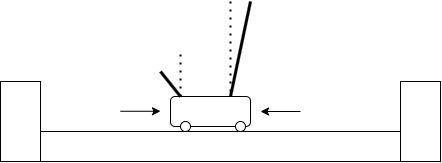
\includegraphics[width=0.5\textwidth]{images/pole_balancing.drawio.png}
    \caption{Ilustrație a problemei double pole balancing. Scopul unui algoritm in cadrul acestui mediu este să miște platforma astfel încât pilonii de pe ea sa nu se răstoarne}
    \label{fig:double_pole}
\end{figure}

Totuși, aceeași problema a fost rezolvat de 5 ori mai rapid de \textbf{Enforced Subpopulations}(ESP)\cite{ESP}, astfel că autorii NEAT si-au propus sa demonstreze un argument mai puternic pentru evoluția structurilor, anume ca modificând atât topologia cat și ponderile putem spori cu mult performanta algoritmilor NE. NEAT poate face asta datorita faptului ca minimizează structurile rețelelor pe tot parcursul algoritmului. 
Au existat pe parcursul timpului mai multe metode de evoluție atât pentru topologiile cat și ponderile rețelelor neuronale, ale căror ideii autorii le-au unit în \cite{NEAT} sub termenul de \textbf{"TWEANS"}(Topology and Weight Evolving Artificial Neural Networks). Pentru dezvoltarea NEAT, Kenneth O. Stanley a adresat un număr de probleme nerezolvate la clasa de algoritmi TWEANS. Înainte de asta ar trebui totuși sa prezentam cum funcționează rețelele neuronale și cum acestea învață.

\section{Rețele Neuronale Artificiale}
În natura, o rețea neuronala reprezinta o rețea de neuroni interconectați, care sunt responsabili de funcționarea sistemului nervos. 
Sunt specializați în transmiterea informației prin semnale electrice și au 4 componente principale, dendritele, corpul celular, axonul și butonii terminali.
\begin{figure}[h]
    \centering
    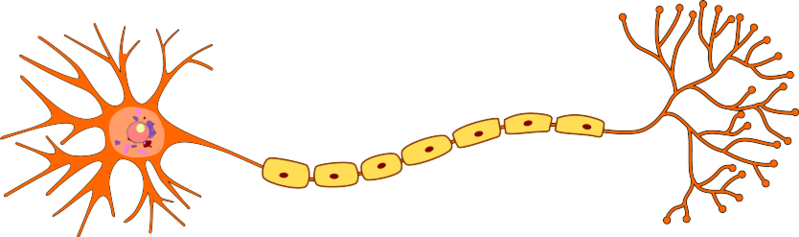
\includegraphics[width=1\textwidth]{images/neuron_structure.png}
    \caption{Structura unui neuron.\cite{Neuron}}
    \label{fig:neuron}
\end{figure}
Fiecare neuron primește informația prin dendrite și le transmite prin axon printr-un semnal electric cu toată puterea sa, dacă a primit destulă informație prin Dendrite. Neuronii sunt conectați intre ei prin sinapse, iar sinapsele își pot adapta numărul de receptori pentru a controla puterea semnalului care vine de la un neuron.
O rețea neuronala artificiala este compusa dintr-o serie de noduri conectate intre ele ca un graf. 
Ca structura, o rețea are un strat de noduri de intrare și  unul de noduri de ieșire, și opțional un număr de straturi ascunse în cadrul rețelelor neuronale profunde.
Fiecare conexiune are o pondere asociata ei ce reprezintă puterea conexiunii. 
Aceste ponderi se pot adapta astfel încât rețeaua sa funcționeze conform așteptărilor. Conform Teoriei Aproximării Universale, o rețea neuronala ar putea sa ajungă aproape de a aproxima orice funcție pentru care este adaptată.
Spre deosebire de creier, într-o rețea neuronala pot exista mai multe tipuri de neuroni, determinați de o funcție de activare. Dacă nu folosim o funcție de activare, valoarea unui neuron este reprezentata de o suma ponderata a intrărilor(Formula \ref{eq:sumaPonderata}) plus opțional un bias al neuronului.

\begin{equation}\label{eq:sumaPonderata}
    z = \sum_{i} w_i x_i + b
\end{equation}

Dacă este folosita o funcție de activare, atunci semnalul nodului va fi outputul funcției de activare, iar input-ul este suma ponderata dintre conexiunile și intrările nodului.
\begin{figure}[h]
    \centering
    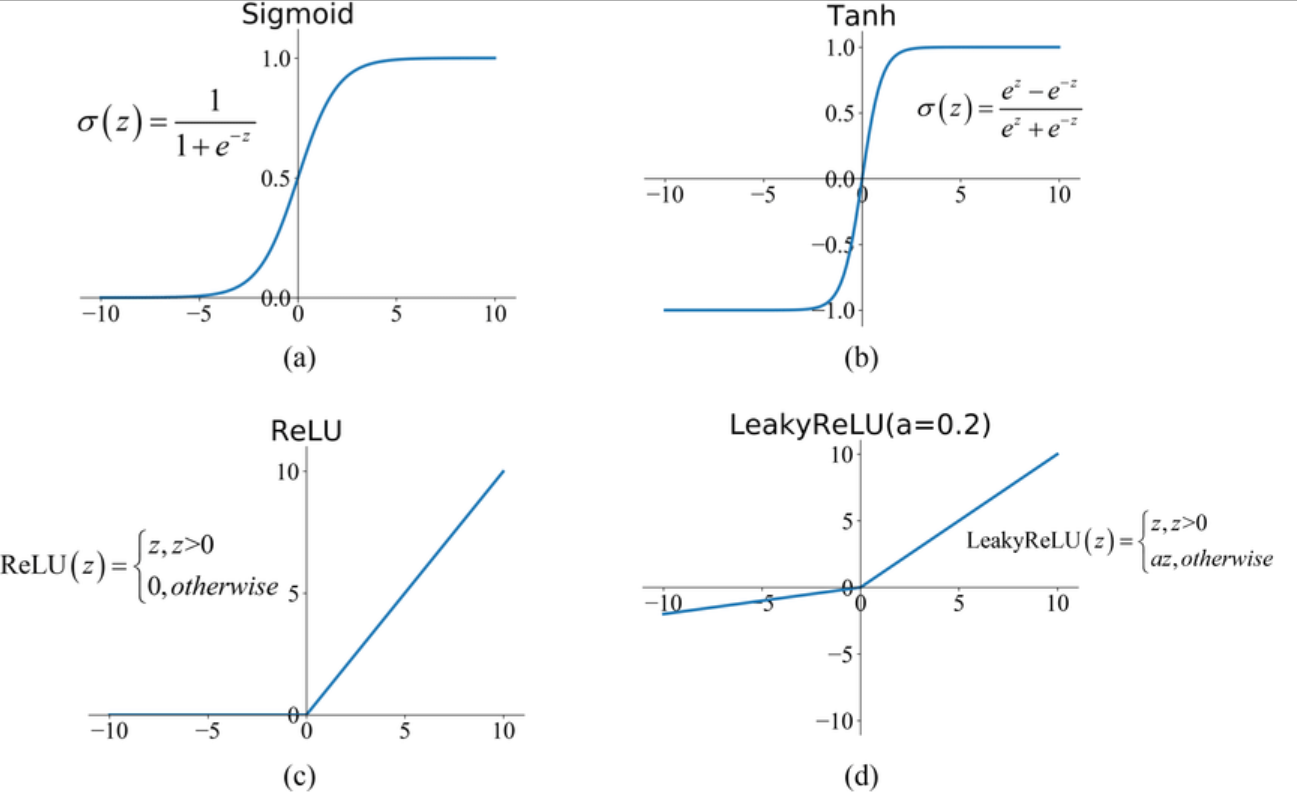
\includegraphics[width=1\textwidth]{images/activation_functions.png}
    \caption{Funcții de activare comune: (a) Sigmoid, (b) Tanh, (c) ReLU, and (d) LReLU.\cite{activation_functions}}
    \label{fig:neuron}
\end{figure}

Rețelele neuronale artificiale tradiționale sunt feedforward, adică datele sunt procesate într-o singura direcție, de la input la output, iar învățarea se face prin algoritmul de backpropagation.
În documentul care descrie NEAT, nu sunt expuse restricții asupra conexiunilor care se pot forma, deci algoritmul poate duce la generarea rețelelor neuronale recurente.
Acestea pot procesa date secvențiale, deoarece conțin conexiuni ciclice, ce se pot forma intre oricare noduri, inclusiv nodul de la care conexiunea a pornit. La fiecare pas de timp, în RNN nodurile procesează atât intrarea curenta cat și ieșirea nodului recurent anterior, ceea ce permite rețelei sa utilizeze informații din trecut.
Pentru antrenare NEAT nu folosește backtracking, ci operatorii genetici.

\section{Problemele în TWEANNs și inovațiile în NEAT}
\subsection{Codificare}\label{Codificare}
O problema pe care trebuie sa o rezolve orice TWEANN este modul în care specificam genomul unui individ. Aici sunt doua categorii mai mari, \textbf{codificare indirecta}  și \textbf{directa}.
Codificarea indirecte de obicei doar specifica reguli pentru crearea fenotipului, și sunt specifice algoritmilor care le folosesc
Pentru codificarea directa opțiunile sunt \textbf{codificarea binara}, care folosește codificare clasica a grafurilor cu șiruri de biți, precum "Structured Genetic Algorithm"(sGA)\cite{sGA}, care reprezinta prin șiruri de biți matricea de conexiuni a rețelei, însa cele mai întâlnite codificări sunt cele de tip graf, care reprezinta grafurile în mod mai explicit.
NEAT folosește o codificare directa, din cauza ca codificările indirecte neavând o mapare directa la fenotip, dacă nu suntem foarte familiari cu procesele genetice, pot perturba căutarea în moduri impredictibile și greu de detectat. Codificarea pe care o alegem este foarte importanta, deoarece aceasta afectează costul operației de crossover, astfel ca exista TWEANNs "nonmating", care nici măcar nu folosesc acest operator\\
Codificarea NEAT a fost proiectata cu scopul de a permite alinierea genom-urilor pentru crossover fără a fi nevoie de o analiza costisitoare a topologiei. Aceasta codificare este reprezentata de o lista de node genes, și o lista de connection genes. Pentru fiecare node gene este specificat id-ul sau și tipul de nod, care clasifica nodurile în noduri de intrare, de ieșire, si noduri ascunse. Primele sunt nodurile de intrare, după care cele de ieșire iar cele hidden sa adaugă la capătul listei în urma mutațiilor.
Fiecare conection gene conține: un in-node și un out-node, care exprima nodurile și direcția conexiunii, ponderea asociata cu conexiunea, o valoare boolean care indica dacă conexiunea ar trebui sa fie exprimata în fenotip, și un număr de inovație(prezentam de ce este necesar în secțiunea \ref{Numar de inovatie}), care permite găsire genelor care corespund din diferiți indivizi și e una din piesele centrale ale algoritmului.
\begin{figure}[h]
    \centering
    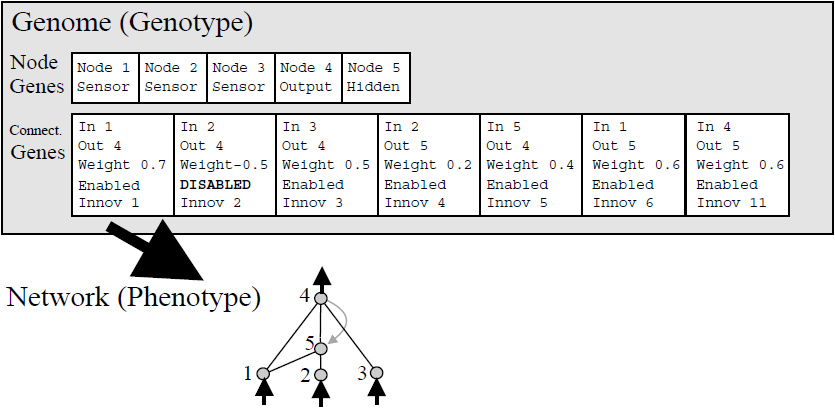
\includegraphics[width=1\textwidth]{images/genotip_fenotip_neat.png}
    \caption{Genotipul in cadrul NEAT si fenotipul(rețeaua neuronala) pe care acesta îl exprima. Figura 2 din \cite{NEAT}},
    \label{fig:encoding}
\end{figure}

\subsection{Inițializarea populației}\label{InitializareNeat}
La majoritatea algoritmilor din clasa TWEANN, populația inițiala este generata cu topologii aleatorii, pentru a asigura diversitate în structurile rețelelor. Totuși, inițializare în modul asta produce multe probleme pentru TWEANNS:
\begin{enumerate}
    \item Nu avem nici o garanție ca informația poate ajunge din fiecare intrare la fiecare ieșire, ceea ce poate face ca unele intrări sa fie irelevante. Timp important de procesare va fi pierdut pentru a scăpa de astfel de rețele.
    \item Ideal am dori ca soluțiile obținute sa fie minime, adică un număr minim de noduri și conexiuni, deoarece o rețea mai complexa necesita mai mult timp pentru optimizarea ponderilor. Cu inițializarea aleatorie, o mare parte din timp ar fi folosita pentru filtrarea structurilor extra care nu ar fi trebuit sa existe de la început. Evaluarea relelor mai complexe ia mai mult timp, dar prin aceasta inițializare nu avem nici o garanție ca soluția va fi minima, deoarece orice rețea atâta timp cat are un fitness mare poate domina peste celelalte.
\end{enumerate}

Soluția NEAT este sa înceapă în mod minim. Populația inițiala are fiecare nod de intrare conectat cu cele de ieșire cu ponderi aleatorii, și nici un nod ascuns, astfel soluția va adăuga structuri noi doar atunci când aceste ajuta la îmbunătățirea fitness-ului. Astfel se asigura minimalitatea nu doar la final dar pe parcursul tuturor generațiilor. Ar trebui sa precizam ca inițial, adăugând unei rețele structuri noi, care nu au fost optimizate, va face ca fitness-ul sa scadă inițial, deci indivizii cu inovații topologice sunt la risc sa dispară, asta fiind un alt motiv pentru care majoritatea algoritmilor TWEANN folosesc inițializarea cu topologii aleatorii. Pentru a evita pierderea inovațiilor, NEAT folsește \textbf{"Speciația"}, pe care o vom detalia în secțiunea \ref{Speciatie}.

\subsection{Problema convențiilor concurente și numerele de inovație}\label{Numar de inovatie}
Problema convențiilor concurente apare atunci când exista mai mult de un singur mod de a reprezenta o rețea neuronala optimizata pentru o problema.
Crossover în cazul a doua astfel de soluții poate duce la pierderea de informație în cadrul noului copil format.
Aceasta problema este încă mai grava în cadrul TWEANNs, deoarece soluții pentru o problema pot fi reprezentate prin topologii complet diferite, iar genomul fiecăreia poate avea lungimi diferite, agravând problema convențiilor concurente. 
Soluția în cadrul NEAT la aceasta problema este inspirata din soluția naturii în cadrul reproducerii sexuale, adică \textbf{omologia}, doua gene fiind omoloage dacă ele sunt trăsături ale aceleiași alele.
NEAT stabilește omologia dintre gene prin intermediul \textbf{marcatorilor istorici}, reprezentați de \textbf{numere de inovație}, care permit stabilirea originii istorice a unei gene, iar astfel putem identifica și genele omoloage.
Vom prezenta cum apar și cum sunt folosite numerele de inovație în secțiunile \ref*{OperatoriGenetici} și \ref*{Speciatie}

\subsection{Operatori Genetici}\label{OperatoriGenetici}
NEAT folosește 2 operatori genetici pentru modificarea genomul-ui indivizilor, mutația și crossover.
Prin mutație, ca și la ceilalți algoritmi de NE, se pot modifica ponderile, prin perturbarea lor sau prin asignarea unei noi valori aleatorii, însa pentru NEAT mutație este și modalitate prin care introducem schimbări structurale.
Sunt folosite 2 tipuri de mutație structurala, "add connection", prin care se adaugă o conexiune cu pondere aleatorie intre oricare 2 noduri care nu erau conectate deja, și "add node", care alege o conexiune în mod aleatoriu, și adaugă un nou nod în locul ei.
Mai exact, conexiunea aleasa este dezactivata, și se creează o noua conexiune intre nodul de intrare al conexiunii dezactivate și nodul nou creat, cu ponderea de 1, iar conexiunea dintre nodul nou și nodul de ieșire primește ponderea celei dezactivate.
Astfel se minimizează efectul inițial al modificărilor structurale, iar ponderile noilor conexiuni vor fi modificate în generațiile viitoare.

De fiecare data când producem o modificare structurala, fiecare gena de conexiune are adăugat și un nou număr de inovație din punct de vedere global.
Acest număr ne permite sa stabilim originea istorica a acestei gene.
Dacă în cursul unei generații, păstram o lista a inovațiilor care au avut loc iar în genomul a 2 indivizi diferiți va apărea o aceeași gena de conexiune, poate doar cu ponderi diferite, aceste gene vor primi ambele același număr de inovație, pentru ca reprezinta aceeași structura dar care a apărut în mod independent în cadrul fiecăreia.
Crossover reprezinta încrucișarea genomului celor 2 părinti, pentru a crea un copil ce are structuri din partea ambilor
Acum, datorita marcatorilor istorici, în cadrul crossover doua genomuri pot fi aliniate după genele care au numere de inovație egale, acestea sunt gene "matching".
Genele care nu sunt matching sunt fie "disjoint" dacă sunt în limita numerelor de inovație a ambilor părinti, fie "excess" dacă unul din părinti are numere de inovații mai mari decât cel mai mare număr al celuilalt părinte.
\begin{figure}[h]
    \centering
    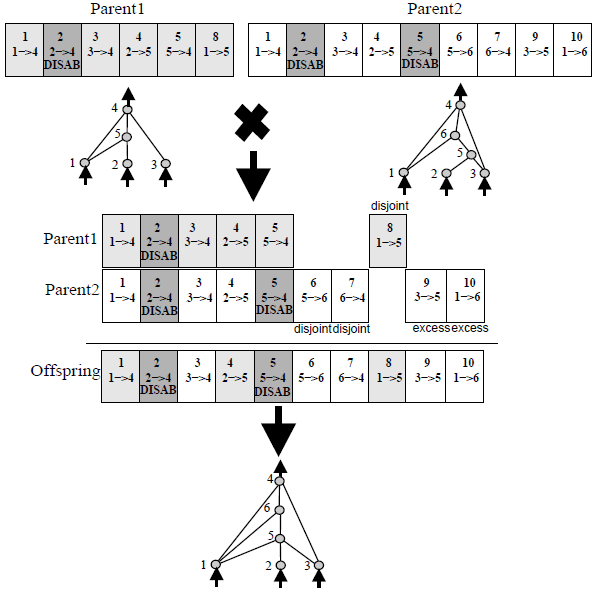
\includegraphics[width=1\textwidth]{images/crossover_matching.png}
    \caption{Procesul de "matching" pentru doua genomuri diferite. Reprezinta figura 4 din \cite{NEAT}}
    \label{fig:crossover}
\end{figure}
În cadrul compunerii copilului, acesta moștenește în mod aleator genele parching ale ambilor părinti, însa doar genele disjoint și excess ale părintelui cu cel mai mare "fitness".
În cazul în care ambii părinti au fitness egal, atunci și genele excess și disjoint sunt moștenite aleator.
Pentru genele dezactivate, este o probabilitate prestabilita ca o gena sa rămână dezactivata dacă ea e asa în cadrul oricăruia dintre părinti.
\\
Prin intermediul acestor 2 operatori genetici, este introdusa diversitate în cadrul populației.
Totuși, de obicei, datorita faptului ca structurile mai mici au mai puține conexiuni, aceste se pot optimiza mai rapid, iar adăugarea de noi structuri, pana acestea sunt optimizate, va scădea din fitness-ul rețelei, deci inevitabil noile inovații ar dispărea rapid dintr-o populație normala, cu tote ca potențial ele ar fi chiar necesare.
Din acest motiv în NEAT este nevoie de \textbf{Speciație}, pe care o prezentam în secțiunea \ref*{Speciatie}.

\subsection{Speciație}\label{Speciatie}
Speciația este un mod de a proteja noile inovații topologice apărute.
Ideea este de a permite indivizilor sa concureze în propria lor nișă, nu cu întreaga populație.
Pentru a detalia, topologiile similare din cadrul populației vor fi încadrate în specii, organismele din aceleași specii concurează în mod principal intre ele, și astfel au timp sa își optimizeze conexiunile.
Cum anume sunt determinate speciile și organismele din cadrul lor? Tot cu ajutorul numerelor de inovație. 
Numărul de gene "desjoint" si "excess" sunt un indicator bun al distantei din punct de vedere al compatibilității intre 2 genomuri.
Astfel, autorii NEAT au ajuns la o formula simpla care sa măsoare compatibilitatea ca o distanta intre 2 structuri diferite în NEAT(notam $\delta$) în termeni de număr de gene excess $E$ și număr de gene desjoint $D$, plus media diferenței dintre genele matching $\overline{W}$:

\begin{equation}\label{eq:compatibility}
    \delta = \frac{c_1 \cdot E}{N} + \frac{c_2 \cdot D}{N} + c_3 \cdot \overline{W} 
\end{equation}

Coeficienții $c_1$, $c_2$ si $c_3$ ajustează importanta acestor factori, iar $N$, care reprezinta numărul de connection genes a genomului cel mai lung, normalizează valorile conform dimensiunii genomului.
Prin calculul valorii $\delta$ putem desfășura procesul de speciație cu ajutorul unei valori stabilite în prealabil, pragul de compatibilitate $\delta_t$.
Procesul de speciație se desfășoară în următorul mod.
Fiecare specie are un genom care o reprezinta. Fie un genom $g$ din generația curenta, acesta este plasat în prima specie cu a cărui reprezentant este compatibil, adică  $\delta < \delta_t$.
Dacă nu exista nici o specie compatibila, se formează una noua cu $g$ ca reprezentat al acesteia.

\subsection{Reproducerea}\label{Reproducerea}
NEAT folosește un mecanism numit \textbf{"explicit fitness sharing"} pentru a evita ca o specie sa devina prea mare și sa ajungă de dimensiunea întregii populații.
Practic, toate organismele din aceeași specie împărtășesc fitness-ul speciei lor.
Fitness-ul ajustat al organismului $i$ este calculat prin formula:

\begin{equation}\label{eq:adjustedFitness}
    f\prime_i  = \frac{f_i}{\sum_{j = 1}^{n}sh(\delta(i,j))}
\end{equation}

unde $f\prime_i$ e fitness-ul ajustat al individului $i$, $n$ e numărul de organisme din populație, iar funcția $sh$ are valoare 0 când $\delta(i, j)$ este peste $\delta_t$, dar 1 altfel.
Astfel, partea de jos a fracției reprezinta doar numărul de indivizi din aceeași specie cu organismul $i$.
Fiecărei specii ii este acordat un număr diferit de membri potențiali depinzând de suma a $f\prime_i$ a membrilor speciei După formula:
\begin{equation}\label{eq:potentialMembers}
    n_k = \frac{\overline{F_k}}{\overline{F_{tot}}} |P|
\end{equation}
unde $k$ reprezinta o specie, $n_k$ e nr de membri asignați speciei, $|P|$ este numărul de indivizi în populație, $\overline{F_k}$ este media fitnessului speciei, adică $\overline{F_k} = \sum_{i}^{} f\prime_i$, iar $\overline{F_{tot}} = \sum_{k}^{} \overline{F_k}$
Întreaga populație este apoi înlocuită de copii membrilor mai buni ai fiecărei specii, membrii mai slabi fiind eliminați în prealabil.
Scopul final al speciației este protejare inovațiilor topologice, iar sistemul întreg cauta o soluție în cel mai rapid mod posibil, deoarece inovații noi apar și sunt păstrate doar atunci când e necesar.

    \chapter{rtNEAT}\label{rtNEAT}

rtNEAT este o metoda bazata pe NEAT(vedeți capitolul \ref*{NEAT}), dezvoltată de aceiași autori plus Bobby D. Bryant\cite*{rtNEAT}.
Acesta este o adaptare a NEAT, gândită pentru jocuri, pentru evoluția rețelelor neuronale în real-time, permițând agenților controlați de ele sa se îmbunătățească în timpul desfășurării jocului.
Pentru a demonstra acest concept de joc, a fost dezvoltat "NERO"(Neuro-Evolving Robotic Operatives)\cite*{NERO}, un joc bazat pe rtNEAT, în care un jucător antrenează o echipa de roboti virtuali pentru a se lupta cu robotii altei echipe.
Una dintre principalele observații care au permis dezvoltarea rtNEAT este faptul ca într-un joc toată populația joaca în același timp, deci fitness-ul este înregistrat constant, astfel agenții de-asemenea s-ar putea adapta constant.
Am considerat acest algoritm potrivit deoarece în mediul nostru virtual, ne dorim ca organismele sa evolueze și sa se adapteze în timp-real, pe baza răspunsurilor pe care le primesc de la diversele interacțiuni cu mediul, astfel am putea vedea o evoluție în termeni de comportamente cat și ca număr de indivizi, deoarece algoritmul NEAT resetează populația la fiecare generație.
\\
În cadrul rtNEAT, la fiecare $n$ intervale de timp, se executa o serie de operațiuni pentru înlocui un organism cu performante scăzute cu copilul dintre 2 organisme mai performante, alese în mod probabilist astfel încât sa prezerveze speciația din NEAT.

\begin{figure}[h]
    \centering
    
\includegraphics[width=0.25\textwidth]{images/logoFii.png}
    \caption{Ciclul de înlocuiri în cadrul rtNEAT}
    \label{fig:crossover}
\end{figure}

\section{Înlocuirea agentului cel mai puțin adaptat}
Prin aceasta operație, se înlocuiește un agent puțin performant cu unul potențial mai performant, dar în asa fel încât se păstreze dinamica de speciație din NEAT.
Pentru asta, alegem sa eliminam agentul cu cel mai mic "fitness ajustat", deoarece dacă alegerea sar face după cel mai rău fitness "neajustat", ar fi eliminate întâi organismele din specii în care a apărut o inovație topologica noua și care nu a avut timp sa se optimizez, astfel speciația nu ar mai proteja inovația.
Fitness-ul ajustat este calculat la fel ca în cadrul NEAT, adică pentru individul $i$, $f\prime_i = \frac{f_i}{|S|}$, $|S|$ fiind numărul de indivizi din aceeași specie cu $i$.
\\
Trebuie de asemenea sa ne asiguram ca fiecare individ a supraviețuit destul înainte sa fie eliminat, deoarece altfel ar fi eliminați mereu cei mai noi indivizi, care nu au avut timp sa acumuleze fitness.
Din acest motiv, rtNEAT elimina doar agenții care au supraviețuit minimul de timp. Acest parametru e setat experimental.
După eliminarea unui agent, este important sa estimam din nou fitnessul mediu $\tilde{F}$, deoarece acesta se schimba, și este folosit în următorul pas al algoritmului.

\section{Generarea copilului}
Din cauza ca nu generam din nou întreaga populație la începutul fiecărei populații, nu poate fi utilizata formula \ref{eq:potentialMembers}, dar dinamica speciației poate fi conservata dacă alegem părintele în mod probabilist:
\begin{equation}\label{eq:chooseParentSpecies}
    Pr(S_k) = \frac{\overline{F_k}}{\overline{F_{tot}}}
\end{equation} 
adică probabilitate de a alege o specie anume pentru părinți este proporționala cu raportul dintre fitness-ul mediu al speciei și suma fitness-urilor medii pentru toate speciile.
Noul copil este format prin crossover dintre 2 indivizi din specia aleasa plus mutația.
\\
Dacă folosim un prag de compatibilitate dinamic $\delta_t$, atunci nu putem face la fel ca în "NEAT", adică sa îl actualizam înainte de crearea următoarei generații, deoarece aproape toată populația va rămâne în aceeași specie.
În rtNEAT, este ales un număr de înlocuiri de indivizi intre care se fac ajustări ale $\delta_t$, de exemplu la fiecare 3 înlocuiri, iar pe baza noului $\delta_t$ fiecare individ din populație va fi repartizata din nou la una speciile existente.

\section{Parametrii de rulare a algoritmului}
Toți Pașii algoritmului rtNEAT, pe care i-am discutat mai sus, trebuie executați la intervale regulate, adică la fiecare $n$ ticuri de timp.
Parametrul $n$ trebuie ales astfel încât rata de înlocuire sa le permită agenților sa supraviețuiască destul cat sa ajungă la timpul minim $m$, pentru a putea fi evaluați, adică sa treacă din statutul de neeligibili pentru înlocuire în eligibili, dar și destul de des cat sa nu se încetinească evoluția la un grad frustrant.
Pentru a determina parametrii potriviți, autorii au stabilit o lege a eligibilității, care stabilește ce proporție din populație ne putem aștepta sa fie neilegibilă odată ce algoritmul a trecut de primele generații când toată populația este neilegibilă:
\begin{equation}\label{eq:Law Of Eligibility}
    I = \frac{m}{|P|n}
\end{equation}
unde $I$ e fracția neilegibilă din populație, $m$ e durata minima de viata pe care o poate avea un individ, $n$ este numărul de ticuri intre procesele de înlocuire, iar $|P|$ numărul de indivizi în populație.
Practic, cu cat este mai mare populația și numărul de ticuri intre înlocuiri, cu atât este mai greu este înlocuită populația în întregime, deci mai putini agenți neeligibili, iar cu cat $m$ este mai mare, cu atât mai multi vor fi sub pragul eligibilității.
Astfel, putem construi o formula pentru $n$:
\begin{equation}\label{eq:formula for n}
    n = \frac{m}{|P|I}
\end{equation}
Astfel, parametri pe care trebuie sa ii alegem noi rămân doar $m$, $|P|$ și $I$.
\\
Procesele descrise pana acum permit rtNEAT sa replice dinamica NEAT, dar în timp real.
    \chapter{Mediul Virtual}\label{MediulVirtual}
În acest capitol vom descrie mediul Unity în care se desfășoară simularea.
O scena în Unity este compusa dintr-o mulțime de \textbf{GameObjects}, care interacționează intre ele în timpul jocului, sau care prezintă doar aspecte estetice.
\begin{wrapfigure}{l}{0.25\textwidth} %this figure will be at the right
	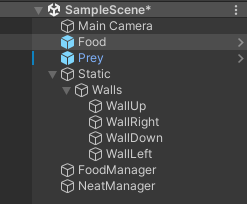
\includegraphics[width=0.25\textwidth]{images/scene_structure.png}
\end{wrapfigure}
Mai departe vom prezenta obiectele din cadrul simulării, proprietăților lor, și cum interacționează cu celelalte obiecte din mediu.
Structura scenei a fost inspirata din proiectul "Simulated Fish Ecosystem"\cite*{ZolphiteNeatYoutube}.

\section{Vizualizarea principala}
În mod implicit, înainte sa dam start oricărei simulări, în mediu avem 2 structuri principale: camera(\textbf{Main Camera}) și pereții(\textbf{Walls}).
\textbf{Main Camera} stabilește dimensiunea \textbf{Game view}-ului (poate fi văzut ca preview în coltul de dreapta jos a  imaginii \ref{fig:mainCameraView}, unde de-asemenea putem vedea cu o linie gri subțire marginea view-ului), cat și culoarea din background.
Pentru view-ul prezentat de camera nu avem o dimensiune standard, deoarece o schimbam depinzând de cantitatea de mâncare și de cate creaturi vrem sa folosim în cadrul unei simulări, însa păstram un aspect de imagine constant de 16:9.
Obiectul "Walls" este compus din 4 pereți(reprezentați ca segmente albe în cadrul imaginii \ref{fig:mainCameraView}): \textbf{WallUp}, \textbf{WallRight}, \textbf{WallDown} si \textbf{WallLeft}.
Aceștia sunt obiecte statice, care nu se mișca în timpul simulărilor.
Dimensiunea lor de asemenea nu este standard, dar la scalare menținem același aspect de imagine precum camera.
Fiecare dintre pereți are atașat un \textbf{Box Collider 2D} care este setat ca fiind Trigger, pentru a detecta coliziunile cu alte obiecte, și un \textbf{Rigidbody 2D} static plus tag-ul "Wall", pentru a putea fi detectați prin intermediul \textbf{Raycast}(detalii în secțiunea \ref{Senzori}).
Atunci când scalam pereții pentru diferite experimente o facem astfel încât marginile interioare ale pereților sa fie în afara marginilor view-ului camerei, deoarece la generarea cu coordonate aleatorii ale mâncării și ale creaturilor, acestea sunt generate intre marginile game view-ului, iar pereții fiind în afara lui evitam generarea obiectelor în pereți.

\begin{figure}[h]
	\centering
	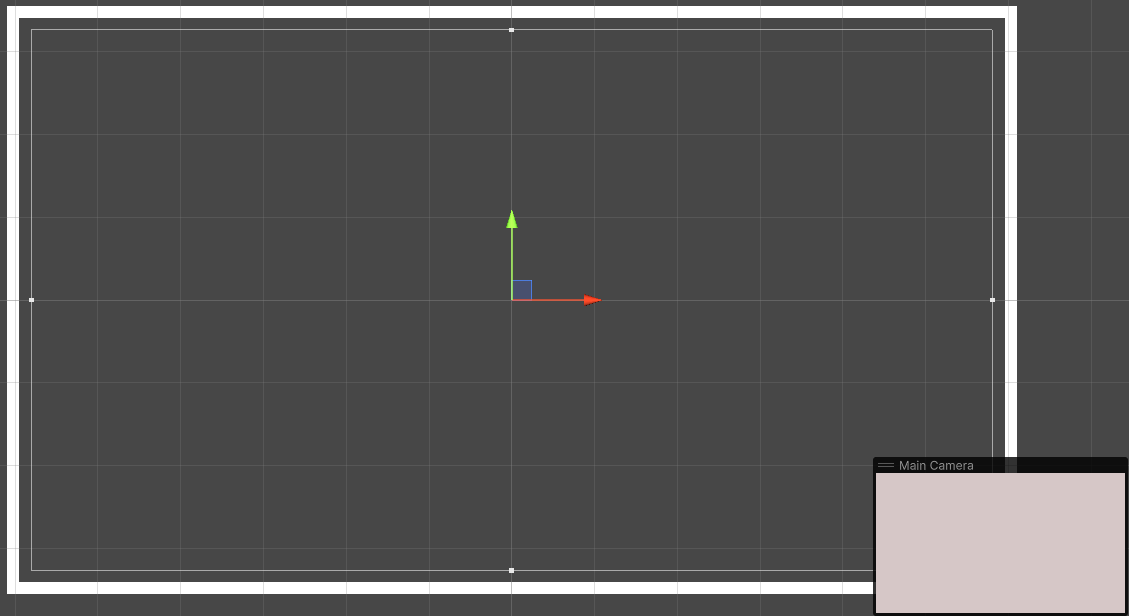
\includegraphics[width=0.75\textwidth]{images/unity_camera-view.png}
	\caption{Main camera view din Unity}
	\label{fig:mainCameraView}
\end{figure}

\section{Mâncarea}
Obiectele din ciclul de generare a mâncării sunt 2, \textbf{Food (Prefab asset)}(componente în imaginea \ref{fig:foodPrefab}) și \textbf{FoodManager}.
\textbf{Food Prefab} reprezinta schema după care se construiește o bucata de energie.
Bucățile de energie se găsesc pe harta sub forma de discuri de culoare galbena, mai exact \#F6F800.
Acestea, ca și pereții, reprezint obiecte statice care odată create nu se mișca.
\textbf{Food Prefab} are asociate următoarele componente:
\begin{itemize}
	\item \textbf{Circle Colider 2D} permite detectarea coliziunilor cu Obiectul
	\item \textbf{Rigidbody 2D} permite ca obiectul sa poată fi lovit de Raycasts
	\item \textbf{Food Controller} un script C\# care controlează distrugerea obiectului.
\end{itemize}
Obiectele construite prin FoodPrefab au scala de 1 pe axa X, Y și Z, și sunt asociate cu tag-ul "Food" pentru a permite detecția lor prin Raycasts și coliziuni.
De asemenea, ele sunt asociate cu \textbf{"Layer"}-ul "Food" pentru a permite detecția lor de către senzorul "Field of View"(secțiunea \ref{Senzori}).
\begin{figure}[h]
	\centering
	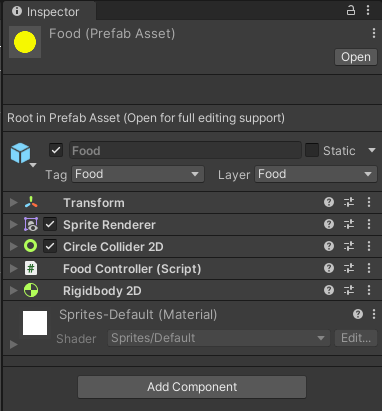
\includegraphics[width=0.5\textwidth]{images/food_prefab.png}
	\caption{Componentele Prefab-ului Food}
	\label{fig:foodPrefab}
\end{figure}

\textbf{FoodManager} este un "Empty Object", al cărui singur scop este sa fie un obiect permanent în aplicație de care putem atașa un script.
Scriptul pentru \textbf{FoodManager} ne permite sa asociem acestuia un "Prefab", în cazul acesta \textbf{Food Prefab}, iar scriptul ne oferă funcții pentru a crea un obiect sau mai multe din "Prefab-ul" asociat, și ne permite și sa le distrugem pe toate.
În \textbf{Food Controller}, scriptul pentru \textbf{FoodPrefab}, funcția "DieAndRespawn" permite distrugerea obiectului Food și regenerarea sa într-o alta locație în mediu, printr-un apel la FoodManger.
Astfel putem păstra numărul de bucăți de energie constant în mediu, chiar dacă energia este colectata în continuu de speciile de prada.

\section{Creaturile}
În mediul nostru virtual avem doua tipuri de creaturi, \textbf{Prada} si \textbf{Pradator}, care pot fi construite prin intermediul \textbf{Prey (Prefab Asset)} și respectiv \textbf{Predator (Prefab Asset)}.
În aceasta vom enunța în mare parte proprietățile pentru \textbf{Prey Prefab}, deoarece cele 2 prefaburi au multe elemente comune, deci pentru \textbf{Predator Prefab} vom expune doar diferențele.
\begin{figure}[h]
	\centering
	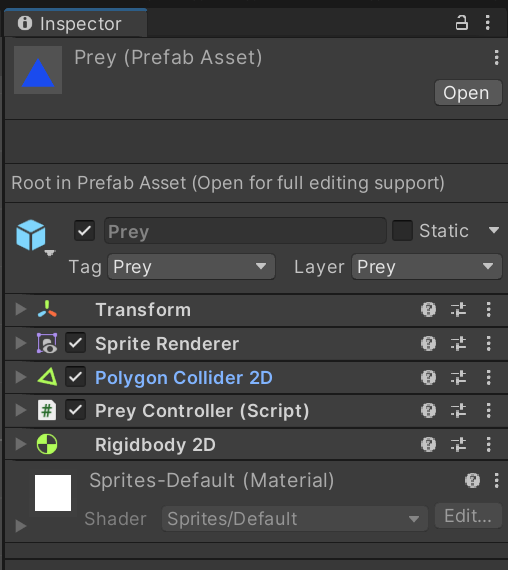
\includegraphics[width=0.5\textwidth]{images/prey_prefab.png}
	\caption{Componentele Prefab-ului Prey}
	\label{fig:preyPrefab}
\end{figure}

Prefab-ul pentru Prey definește următoarele componente:
\begin{itemize}
    \item \textbf{Sprite Renderer}: Definim forma creaturilor prey ca fiind un triunghi, scalat la dimensiunea de 1.5 pe axa x si Y
    \item \textbf{Polygon Collider 2D}: Un Collider care ia forma sprite-ului, folosit pentru detectarea coeziunilor
    \item \textbf{Rigidbody 2D}: Necesar pentru detectarea coliziunilor, pentru ca detectarea coeziunilor se va face în cadrul obiectelor dinamice: Prey si Predator. 
    Este de tip "Kinematic", spre deosebire de static pentru obiectele statice, și permite detectarea coeziunilor kineamtic/static și kinematic/kinematic.
    \item \textbf{Prey Controller}: script C\#, moștenește clasa \textbf{Creature Controller}, care încapsulează trăsături comune atât pentru prey cat și pentru predator, definește mișcarea, senzorii, acumularea de energie și moartea obiecte Prey.
\end{itemize}

\subsection*{Mișcarea}
Mișcarea este definita de schimbări care au loc asupra vitezei și a unghiului de rotație al creaturii. O creatura se poate deplasa doar în fata sau în spate, dar aplicând rotații asupra proprietății "transform.eulerAngles" se poate schimba direcția în care aceasta merge.
Schimbările asupra vitezei și a rotației obiectului sunt determinate de o rețea neuronala asociata obiectului, care primește ca input un număr de valori senzor, și returnează doua valori în intervalul (-1, 1), prima fiind modificarea asupra accelerației iar a doua modificarea asupra rotației.
Acest proces are loc în funcția "FixedUpdate()", deci la fiecare schimbare de frame stratul de intrare se încarcă cu valorile senzorilor, se executa pasul de feed-forward iar valorile din stratul de ieșire sunt folosite pentru a modifica poziția creaturii.

\subsection*{Senzori}\label{Senzori}
În mod implicit, toate creaturile au următorii senzori:
\begin{itemize}
    \item \textbf{Bias}: este un senzor care are mereu valoarea 1, folosit pentru a adăuga bias la nodurile care creează o conexiune cu el.
    \item \textbf{Perete}: acesta este un singur senzor, definit de un Raycast în fata obiectului(în planul 2D, aceasta reprezinta direcția "up" pentru proprietatea "transform" a obiectului). 
    Un raycast reprezinta proiectarea unei raze invizibile de o anumita lungime dintr-un punct, pe o direcție in scena.
    Când aceasta lovește collider-ul unui alt obiect din scena, este returnat un obiect din clasa "RaycastHit2D"(pentru mediul nostru 2D), care poate fi analizat pentru a determina ce tip de obiect a fost lovit(prin intermediul tag-ului) obiectului, și distanta de la punctul de pornire la care a fost lovit.
    Pentru senzorul de pereți, dacă raycast-ul lovește un perete, valoarea sa va fi raportul dintre distanta pana la lovitura și lungimea razei(deci, intre 0 și 1). Dacă nu a fost detectat un perete, valoarea senzorului e 1.  
    \item \textbf{Viteza curenta}: valoarea senzorului este valoarea precedenta a ieșirii pentru "viteza" a rețelei neuronale.
    \item \textbf{Unghi}: unghiul curent, exprimat intre -1 și 1, dintre direcția înainte a creaturii și axa $Y$ a scenei.
\end{itemize}
Pentru detecția țintelor creaturilor(adică a surselor de energie pentru fiecare tip în parte, prădătorii detectează creaturi de tipul prada, iar prada detectează bucățile de energie), am folosit în timp 2 tipuri de senzori.
Cel mai simplu reprezinta un sistem format din 3 Raycast-uri, o sa îl numim \textbf{fork} pentru a ne referi la el mai departe, care acționează la fel ca senzorul implicit pentru perete, doar ca în loc sa detecteze pereți, detectează țintele creaturii.
Un raycast este proiectat pe direcția înainte a obiectului, iar celelalte doua la un unghi de $45^{\circ}$ respectiv $-45^{\circ}$ fata de aceeași direcție.
\\
Ulterior am dezvoltat un senzor mai complex, de tip "Field of View", al cărui concept vine din \cite{rtNEAT}, secțiunea 5, figure 10, unde sunt descriși mai multi senzori printre care și "Enemy Radars".
Acesta descrie divizarea spațiului de $360^{\circ}$ din jurul agentului în mai multe zone. Fiecare zona activează un senzor în dependenta de cat de apropiat este un inamic de agent. Dacă sunt mai multi inamici în aceeași zona, se sumează activările pentru fiecare inamic în parte.
\begin{figure}[ht]
	\centering
	\animategraphics[autoplay,loop,width=\textwidth]{20}{images/sensors_showcase/sensors_showcase-}{9}{111}
	\caption{Senzorul FoV si senzorul pentru perete din cadrul prazii, liniile colorate arata distnata pana la fragmentele de energie care sunt detectate de diferitele zone ale senzorului. Linia alba atunci cand prada se apropie de perete este raycast-ul catre perete}
    \label{fig:senzorDemo}
\end{figure}

În cadrul implementării noastre, pentru senzorul "Field of View"(\textbf{FoV}), alegem un unghi, intre 0 și 180 de grade, care reprezinta câmpul vizual din fata unei creaturi, și raza pana la care acesta se extinde.
Prin alt parametru, specificam în cate zone se împarte acesta. 
Prin intermediul metodei "Physics2D.OverlapCircleAll", se detectează toate țintele din cadrul unui cerc din jurul creaturii, după care, analizând unghiul dintre direcția înainte a creaturii și poziția unei ținte, putem determina dacă țintele cad în cadrul câmpului vizual, și în ce zona a câmpului.
Pentru fiecare zona, activarea ei va reprezenta valoarea calculului $\sum_{i} 1 - d_i/r$, $i$ fiind o ținta din cadrul zonei, $d_i$ distanta pana la ținta, iar $r$ raza cercului în care are loc detecția. Deci pentru fiecare ținta avem o activarea intre 0 și 1, care este mai mare cu cat ținta e mai aproape de creatura.
În cadrul animației \ref{fig:senzorDemo}, se poate vedea cum funcționează senzorul "FoW", cu un câmp vizual de $90^{\circ}$, împărțit în 3 zone, pe o distanta de 20 "world units", iar la sfârșitul animație putem vedea și o vizualizare a raycast-ului pentru senzorul de perete.
Pentru a scrie vizualizarea în "Editor View" a senzorului "FoW" un mare ajutor a fost \cite{FoWVisualization}.
În unul din experimentele de la capitolul \ref{Rezultate}, vom arata ca prada care folosește senzorul "FoW" este superioara celei care folosește "Fork", și vom prezenta și diferențele de comportament intre cele 2 tipuri de prada.
Pentru prădătorii la senzori nu se schimba nimic decât țintele căutate, acestea fiind creaturile de prada.

\subsection*{Coliziuni}
Datorita faptului ca toate obiectele care interacționează în cadrul scenei au asociat cate un collider și un rigidbody, putem detecta coliziunile intre ele.
Procesare acestor coliziuni se face în cadrul script-uri-lor "Prey Controller" și "Predator Controller", asociate prefab-ului "Prey" și respectiv "Predator".
Prin intermediul tag-urilor "Wall" și "Food", script-ul "Prey Controller" înregistrează coliziunile cu pereții, ceea ce cauzează moartea prăzii, și coliziunea cu fragmentele de energie, prin care energia asociata fragmentului este absorbita, iar fragmentul prin funcția "DieAndRespawn" este regenerat la alte coordonate aleatorii în cadrul scenei, deci cantitatea de energie în scena este constanta.
Procesare coliziunilor prada-prădător are loc în script-ul "Predator Controller", și pot fi identificate prin tag-ul asociat creaturilor de prada, "Prey". În cadrul acestor coliziuni, obiectul prada este distrus, însa obiectul prădător primește energie, într-o cantitate semnificativ mai mare decât ce primesc creaturile prada la coliziunile prada-fragment de energie, plus un procent din energia acumulata de prada de-a lungul vieții.
Facem aceste ajustări deoarece vânatul pentru prada este mult mai ușor decât cel pentru prădător,pentru ca prădătorii trebuie sa dezvolte comportamente de chassing, astfel ca prădătorii ar trebui sa primească mai multa energie din vânat pentru a ne asigura ca aceștia nu sunt surclasați de prada în cadrul evoluției.
Coeziunile prădător-perete sunt la fel ca la prada, însa prădătorii nu înregistrează coliziunile cu fragmentele de energie, deoarece vrem ca aceștia sa obțină energie doar prin coliziunile cu prada.
Pe tot parcursul vieții lor, creaturile consuma energie în mod constant, plus o cantitate care depinde de viteza cu care se mișca. Astfel le încurajam sa acumuleze energie încontinuu.
Odată ce o creatura rămâne fără energie, aceasta moare.

\section{Managementul Algoritmului}
\textbf{NeatManager}, ca și FoodManger, este un "Empty Object" pe care îl folosim pentru a atașa script-ul "Neat Manager".
Acest script este responsabil de desfășurare algoritmului Neat, deci are ca responsabilități generarea populației inițiale, înregistrarea morților, crearea generațiilor următoare și înregistrarea de log-uri despre populație pe parcursul generațiilor.
În cadrul NeatManager putem decide sa efectuam experimente în care folosim doar creaturile de prada, sau și prădătorii, și putem determina parametri cum ar fi numărul de membri, numărul de noduri pentru stratul de intrare cat și cel de ieșire etc.(vom discuta mai pe larg mulțimea de parametri în secțiunea \ref{SetariExperimentale}). 
Faza de generare a populației inițiale se desfășoară în următorul mod:
\begin{enumerate}
    \item Se generează genomul inițial pentru fiecare membru din populație(reprezinta o codificare Neat a unei rețele cu structura minima dar cu ponderi ale conexiunilor aleatorii, revedeți secțiunea \ref{InitializareNeat})
    \item Se generează fenotipul pentru fiecare genotip(rețeaua neuronala propriu-zisa, vom expune maparea de la fenotip la genotip în capitolul \ref{DetaliiImplementare})
    \item Se creează agenții simulării, După prefab-ul care a fost asignat către NeatManager. Proprietățile acestora sunt setate După parametrii NeatManager pentru un prefab specific, și sunt poziționați la coordonate aleatorii în cadrul "Main Camera View", fiecăruia dintre ei fiindu-i asignata și una dintre rețele create la pasul precedent.
\end{enumerate}
După creare, agenții sunt liberi sa exploreze mediul și sa acumuleze fitness. În secțiunea anterioara nu am menționat ca în toate scenariile în care un agent moare, asta fiind valabil atât pentru prada cat și pentru prădători, acesta își înregistrează moartea și cauza ei la "NeatManager", prin intermediul funcției "RegisterDeath".
Astfel, NeatManager poate determina când toți agenții din mediu au fost distruși, și poate începe crearea următoarei generații.
Înainte de crearea următoarei generații, se log-eaza fitness-ul average și fitness-ul celui mai bun agent din generația curenta, plus informații despre structura celui mai bun agent.
Procesul de generare a următoarei generații decurge la fel ca cel de inițializare, doar ca mai întâi se aplica o filtrare pentru a rămâne doar genom-urile cele mai bune din cadrul fiecărei specii, care vor trece prin procesul de crossover și de mutație pentru generarea genomurilor generației viitoare.
Aceste genom-uri sunt asignate către diferite specii din populație, care grupează genomuri similare. După acest pas se creează noile rețele neuronale, și se generează noii agenți care gândesc prin intermediul  acestora, iar tot procesul se repeta din nou la fiecare generație.
Ne-am permis în aceasta secțiune sa facem un rezumat al funcționarii algoritmului, vorbind despre obiectul care este responsabil de desfășurarea lui, însa în capitolul \ref{DetaliiImplementare} vom expune detaliat, cu exemple din cod, procesele din cadrul algoritmului.

    \chapter{Detalii de implementare}\label{DetaliiImplementare}

\begin{lstlisting}[caption={Test caption}]
    private void CreateNewSpecies(int genomeIdx)
    {
        var s = new Species(speciesId++);
        s.MembersIdx.Add(genomeIdx);
        s.SpeciesRepresentative = allGenomes[genomeIdx];
        species.Add(s);
        Debug.Log($"<color=#{s.GetStringColor()}>New Species created with id {s.Id}</color>");
    }
\end{lstlisting}
    \chapter{Parametrii experimentali}\label{SetariExperimentale}
In acest capitol vom descrie in primul rand parametrii tuturor obiectelor din cadrul scenei care pot influenta simularea.
Ulterior vom descrie setul de simulari, scopul fiecareia, si setul de parametri care le definesc.
\section{Main Camera si Walls}
\begin{itemize}
    \item \texttt{Size} : schimba marimea GameView-ului prezentat de camera, si deci schimba si marimea zonei in care se genereaza fragmente de energie si creaturi.
    \item \texttt{Wall transform}: peretii doar trebuie scalati si repozitionati astfel incat sa inchida complet spatiul din interior, dar sa fie putin inafara view-ului camerei principale.
\end{itemize}

\section{FoodManager}
\begin{itemize}
    \item \texttt{Food Prefab}: prefab-ul obiectului ce va fi folosit pe post de mancare
    \item \texttt{Total Food}: numar intreg ce reprezinta cate obiect Food Prefab vor fi generate si pozitionate in scena. Acest numar ramane constant pe parcursul unei simulari.
\end{itemize}

\section{Prey si Predator}
\begin{itemize}
    \item \texttt{Acceleration Factor}: un factor ce scaleaza viteza unei creaturi, care in mod implicit e intre -1 si 1.
    \item \texttt{Turn Factor}: cu cate grade se poate roti o creatura intr-o directie.
    \item \texttt{Smoothing Factor}: factor ce afecteaza fluiditatea miscarilor, atat a rotatiilor cat si a deplasarilor inainte si inapoi.
    \item \texttt{Network}: reteau atribuita creaturii.
    \item \texttt{InputNodes}: numarul de noduri din stratul de intrarea al retelei.
    \item \texttt{OutputNodes}: numarul de noduri din stratul de iesire al retelei.
    \item \texttt{Total Energy}: cantitate de energie atribuita creaturii initial.
    \item \texttt{Energy For Food}: cata energie este obtinuta la coliziunea cu o sursa de mancare.
    \item \texttt{Speed Consumption Multiplier}: un factor ce scaleaza consumul de energie al creaturii in dependenta de viteza cu care aceasta se misca.
    \item \texttt{View Distance}: parametru al senzorului "FoW", stabileste raza din jurul creaturii in care se pot detecta tintele.
    \item \texttt{View Angle}: parametru al "FoW", stabileste unghiul din fata creaturii in care sunt detecatate tintele.
    \item \texttt{Angle Splits}: parametru al "FoW", stabileste in cate zone egale de detectie este impartit \textbf{View Angle}.
    \item \texttt{Fow Targets Mask}: parametru al "FoW", stabileste pe ce Layer va avea loc detectia, adica care sunt tintele senzorului.
    \item \texttt{Wall Ray Distance}: parametru al senzorului de detectie a peretelui, stabileste distanta pe care este proiectat Raycast-ul.
    \item \texttt{Sprite Color}: culoarea sprite-ului atasat creaturii.
\end{itemize}

\section{NeatManager}
\begin{itemize}
    \item \texttt{Creature Prefab}: Prefab-ul din care se vor construi membrii popoulatiei
    \item \texttt{Input Nodes}: numarul de noduri pentru stratul de intrare al retelelor
    \item \texttt{Output Nodes}: numarul de noduri pentru stratul de intrare al retelelor
    \item \texttt{Init Weight Range}: valoare $x$ care defineste intervalul [$-x$, $x$], intre care vor fi initializate ponderile retelelor.
    \item \texttt{Mutation Prob}: probabilitatea ca un genom sa sufere mutatii la aplicare operatorului de mutatie.
    \item \texttt{Weight Perturbance Prob}: probabilitate $p$ a fiecarei gene de conexiune din genom de a suferi o perturbare. Probabilitate ca unei ponderi sa ii fie reatribuite o valoare aleatorie e $1-p$.
    \item \texttt{Perturbance Range}: valoare $x$ care defineste intervalul [$-x$, $x$], intre care se alege o valoare aleatorie pentru perturbarea unei ponderi.
    \item \texttt{Reassignment Range}: valoare $x$ care defineste intervalul [$-x$, $x$], intre care se alege o valoare aleatorie folosita pentru resetarea ponderii.
    \item \texttt{New Node Prob}: probabilitatea ca unui genom sa ii fie aplicat mutatia structurala de adaugare a unui nou nod.
    \item \texttt{New Connection Prob}: probabilitatea ca unui genom sa ii fie aplicat mutatia structurala de adaugare a unei noi conexiuni.
    \item \texttt{Inherid Disabled Gene Prob}: probabilitatea in cadrul crossover, daca una dintre doua gene aliniate "matching" este dezactivat, copilul va mosteni o gena dezactivata.
    \item \texttt{Chance Mutation No Crossover}: probabilitate ca un nou membru din populatie sa nu fie generat prin crossover, ci doar prin operatorul de mutatie aplicat nodului parinte
    \item \texttt{Inter Species Mating Rate}: probabilitate in timpul ca operatii de crossover ca al doilea parinte sa fie ales dintr-o specie aleatorie
    \item \texttt{Species Dropoff Age}: numarul de generatii pe care o specie il poate supravetui daca aceasta nu prezinta imbunatatiri ale fitness-ului celui mai bun membru.
    \item \texttt{Survival Treshold}: procentul din membrii cei mai buni ai unei specii care sunt pastrati pentru crearea genom-urilor populatiei din generatia viitoare.
    \item \texttt{Species Target Count}: Numarul tinta de specii in cadrul populatiei.
    \item \texttt{Compatibility Treshold}: pragul de compatibilitate $\delta_t$. Daca distanta de compatibilitate dintre doua genom-uri este mai mare decat aceasta valoare, atunci genom-urile fac parte din specii diferite.
    \item \texttt{Min Compatibility Treshold}: valoarea minima pentru pragul de compatibilitate
    \item \texttt{Max Compatibility Treshold}: valoarea maxima a pragului de compatibilitate
    \item \texttt{Compatibility Modif}: valoare cu care este modificat pragul de compatibilitate, daca suntem sub numarul tinta de specii, $\delta_t$ va scadea cu atat la fiecare generatie, iar daca suntem peste numarul tinta, $\delta_t$ va creste cu atat.
    \item \texttt{Excess Coef}: valoarea $c1$ din formula \ref{eq:compatibility}
    \item \texttt{Disjoint Coef}: valoarea $c2$ din formula \ref{eq:compatibility}
    \item \texttt{Weight Diff Coef}: valoarea $c3$ din formula \ref{eq:compatibility}
    \item \texttt{Top Members Selection Cutoff}: daca o specie are mai mult de atatia membri, atunci genomul celui mai bun membru al speciei va trece in urmatoarea generatie fara ai fi aplicati operatorii de crossover sau de mutatie.
    \item \texttt{Starting Energy}: cantitatea de energie cu care incepe fiecare membru din populatie.
    \item \texttt{Energy For Food}: cata energie este obtinuta la coliziunea creaturii cu o sursa de mancare.
    \item \texttt{Starting Population}: cate creaturi sunt in populatia initiala a fiecarei generatii.
\end{itemize}
    \chapter{Rezultate}\label{Rezultate}
\section{Rezultate Experiment: comparație senzori "Fork" și "FoW"}\label{ResultsFowVsFork}
În Fig.\ref{fig:averageFoW} și Fig.\ref{fig:averageFork} putem vedea cum progresează fitness-ul mediu al populației (cu roșu) și fitness-ul celui mai bun individ din populație (cu albastru).
Aceste prime date servesc ca un proof of concept pentru faptul că algoritmul NEAT este capabil să dezvolte în populația de pradă comportamente care îi măresc fitness-ul pe parcursul evoluției (colectarea fragmentelor de energie și evitarea pereților), deoarece observăm o creștere atât a fitness-ului mediu cât și cel al celui mai bun membru din populație.
Totuși, din cele două tipuri de senzori, "FoW" se arată a fi cel mai bun, chiar dacă media este similară cu cea a populației care folosește "Fork". Fitness-ul maxim atins de creaturile cu senzor "FoW" este mai mare, ceea ce ne arată că acestea au un potențial mai mare pentru evoluție.
Pe lângă asta, putem observa în Fig.\ref{fig:connectionsFow} și Fig.\ref{fig:connectionsFork} faptul că numărul de conexiuni pentru cel mai bun membru din populația ce folosește "FoW" în ultimele generații este mai mare decât pentru populația "Fork", deci s-ar putea ca senzorul "FoW" să beneficieze mai mult de pe urma adăugării de structuri noi.

\begin{figure}[h]
	\centering
	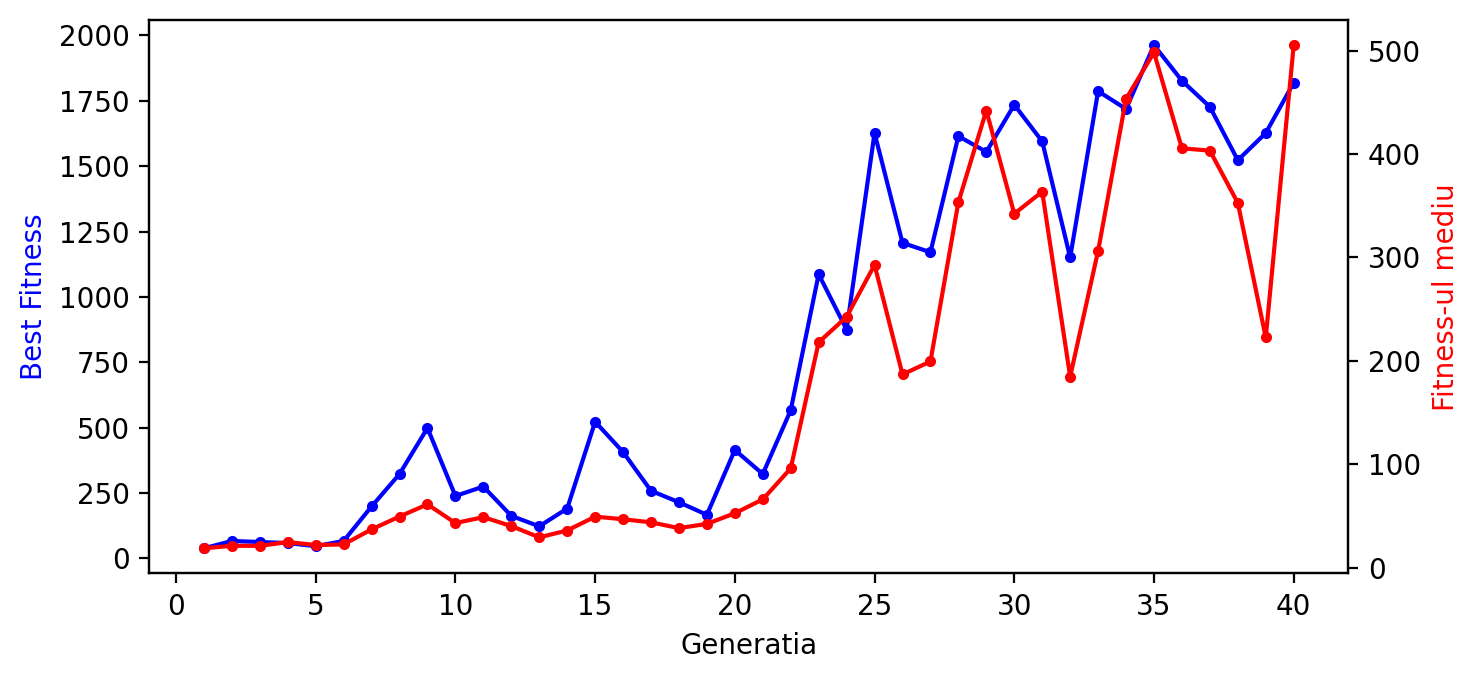
\includegraphics[width=1\textwidth]{images/experiment_fow_average.png}
	\caption{Progresia fitness-ului celui mai bun membru si a fitnessului mediu a populației pe parcursul generațiilor, pentru populații dotate cu senzorul "FoW"}
	\label{fig:averageFoW}
\end{figure}
\begin{figure}[h]
	\centering
	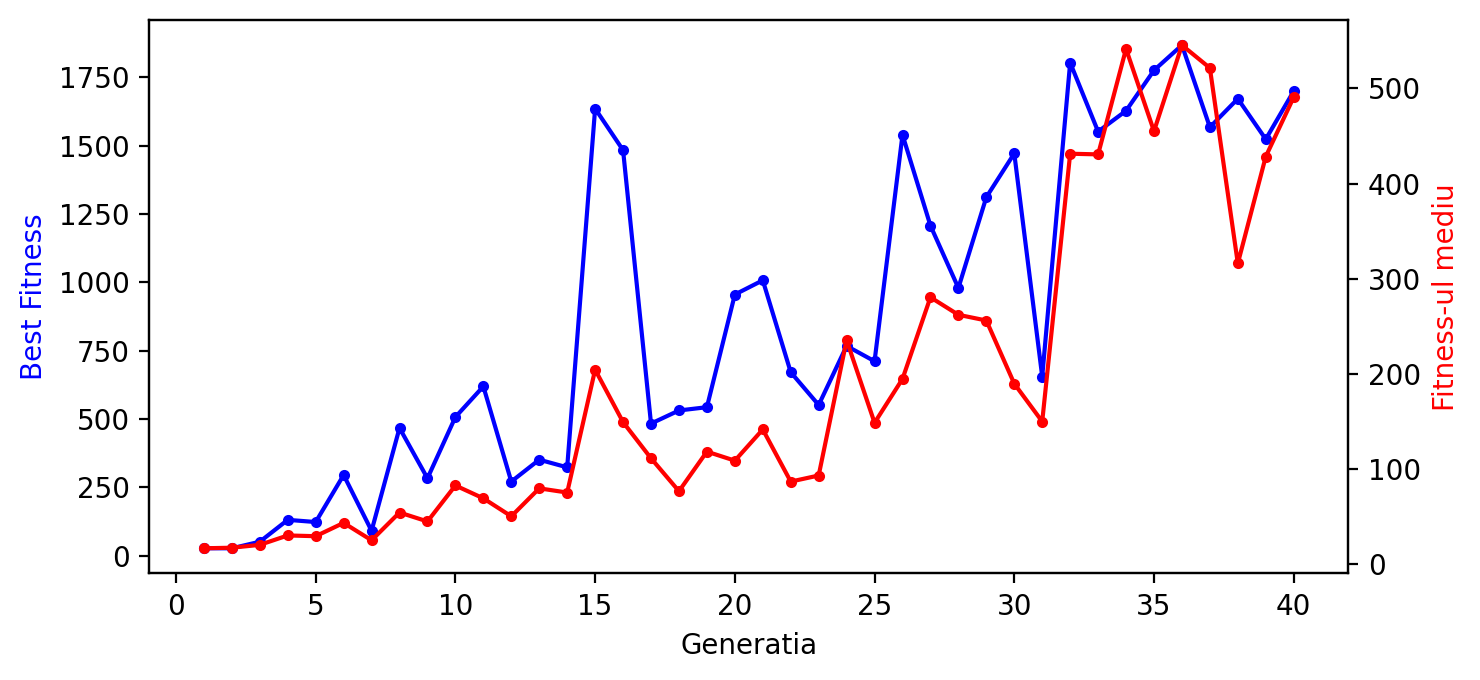
\includegraphics[width=1\textwidth]{images/experiment_fork_average.png}
	\caption{Progresia fitness-ului celui mai bun membru si a fitnessului mediu a populației pe parcursul generațiilor, pentru populații dotate cu senzorul "Fork"}
	\label{fig:averageFork}
\end{figure}
\begin{figure}[h]
	\centering
	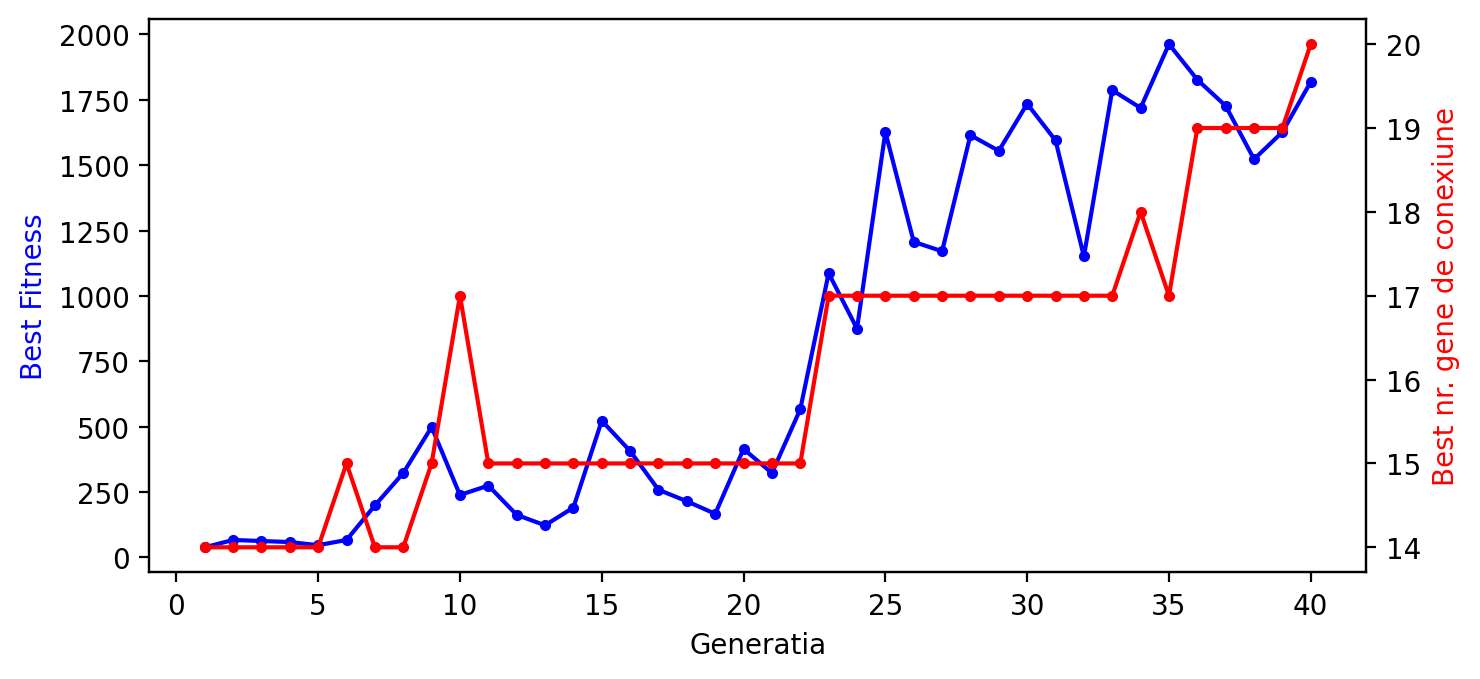
\includegraphics[width=1\textwidth]{images/experiment_fow_connections.png}
	\caption{Progresia fitness-ului celui mai bun membru si a numarului sau de gene de conexiune, pentru populații dotate cu senzorul "FoW"}
	\label{fig:connectionsFow}
\end{figure}
\begin{figure}[h]
	\centering
	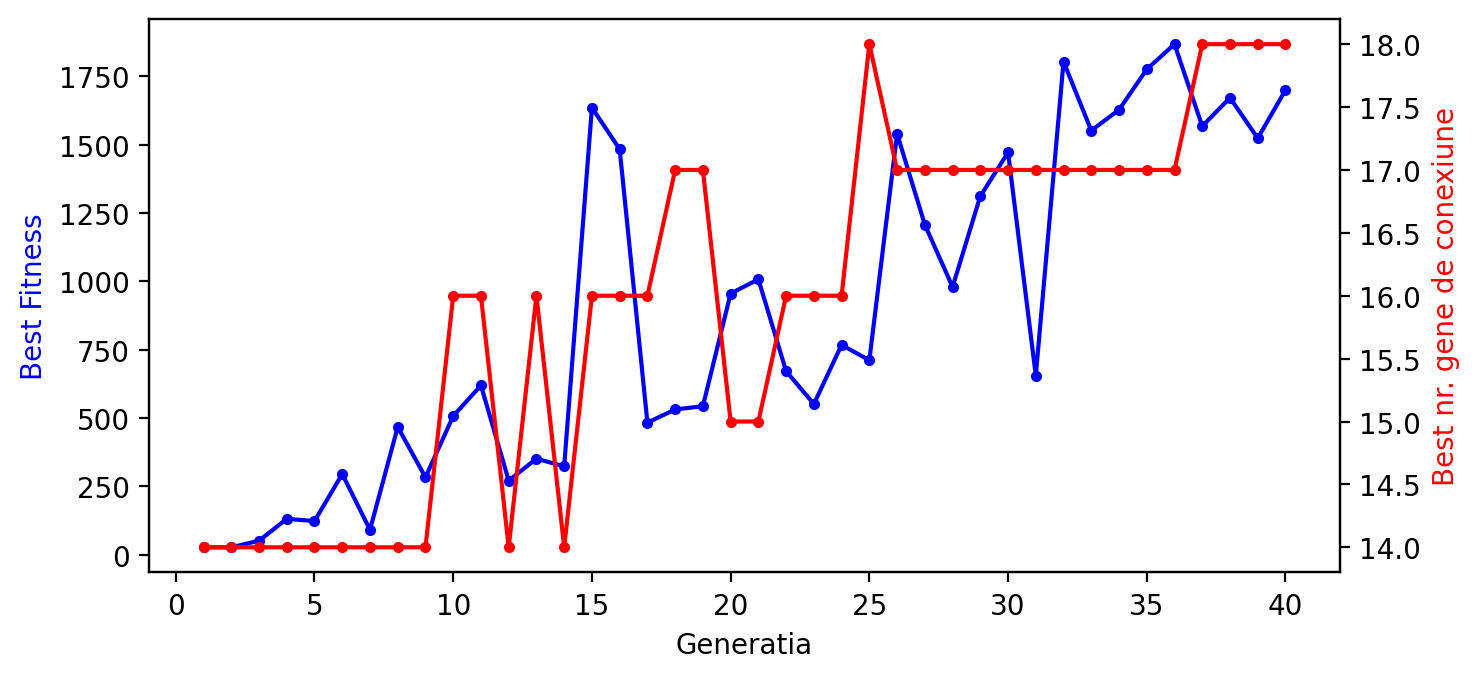
\includegraphics[width=1\textwidth]{images/experiment_fork_connections.png}
	\caption{Progresia fitness-ului celui mai bun membru si a numarului sau de gene de conexiune, pentru populații dotate cu senzorul "Fork"}
	\label{fig:connectionsFow}
\end{figure}

\section{Rezultate Experiment: comparație între păstrarea numerelor de inovație permanent sau resetarea lor la fiecare generație}\label{ResultsPermanentVsReset}
Rezultatele din această secțiune sunt pentru configurarea algoritmului în care lista numerelor de inovație este golită la începutul fiecărei generații, adică nu avem informații despre inovațiile create în generațiile anterioare.
Rezultatele pentru scenariul în care inovațiile sunt păstrate permanent le vedem în secțiunea anterioară, Fig.\ref{fig:averageFoW} și Fig.\ref{fig:connectionsFow}.
Rezultatele ne-au surprins, deoarece presupuneam că scenariul de păstrare în mod permanent al inovațiilor va duce la mai puține specii care sunt mai optimizate și consecvente.
Totuși, din Fig.\ref{fig:averageFoW} și Fig.\ref{fig:averageInov}, se vede clar că atât valorile fitness-ului mediu cât și ale celui mai bun membru sunt mai mari în scenariul curent, nu în cel precedent.
Pe lângă asta, aceste rezultate se ating și printr-un număr de conexiuni mai mic, după cum vedem în Fig.~\ref{fig:connectionsFow} și \ref{fig:connectionsInov}.
Putem presupune că rezultatele arată astfel din cauza că, chiar dacă păstrăm inovațiile timp de mai multe generații, aceeași conexiune în cadrul unei generații și în cadrul alteia s-ar putea să conecteze structuri complet diferite, deci nu ar fi potrivit să le considerăm "matching", dar asta are loc în scenariul păstrării permanente a inovațiilor.

\begin{figure}[h]
	\centering
	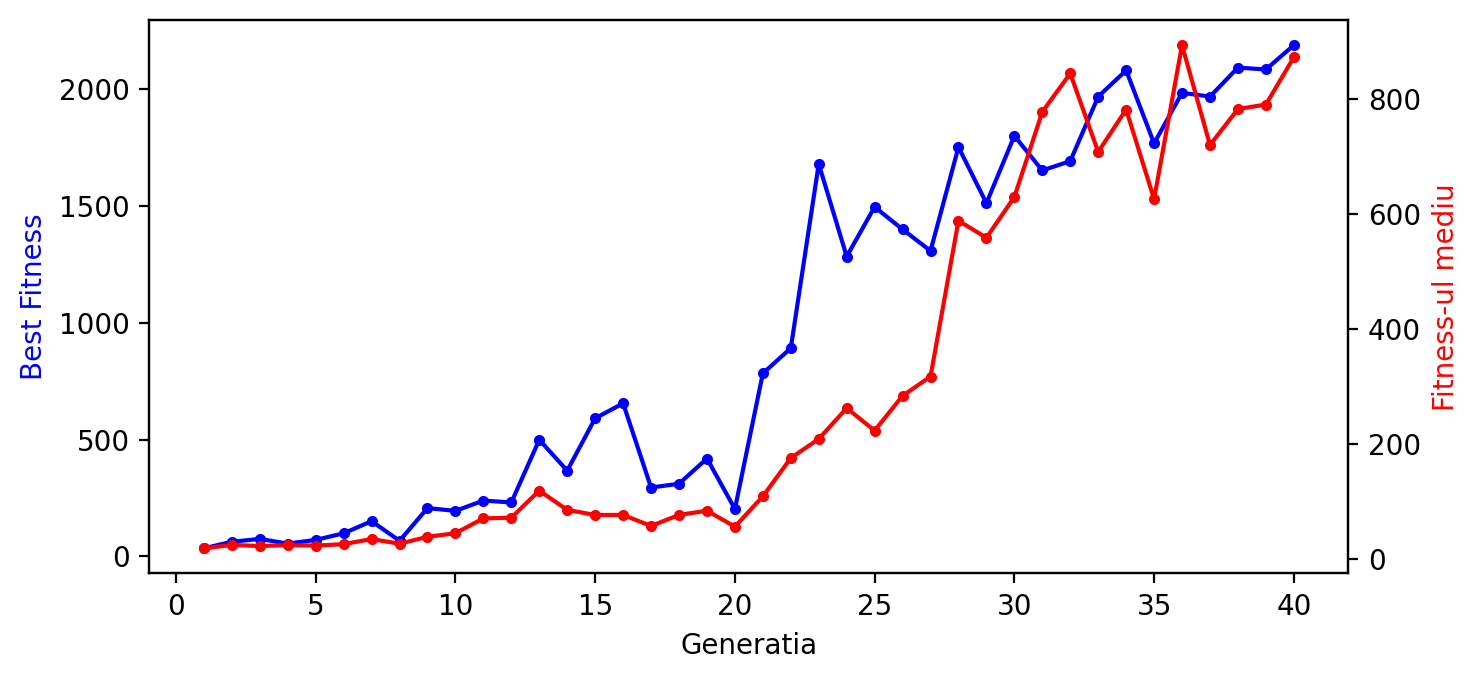
\includegraphics[width=1\textwidth]{images/experiment_inov_average.png}
	\caption{Progresia fitness-ului celui mai bun membru si a fitnessului mediu a populației pe parcursul generațiilor, in scenariul resetării numerelor de inovație}
	\label{fig:averageInov}
\end{figure}

\begin{figure}[h]
	\centering
	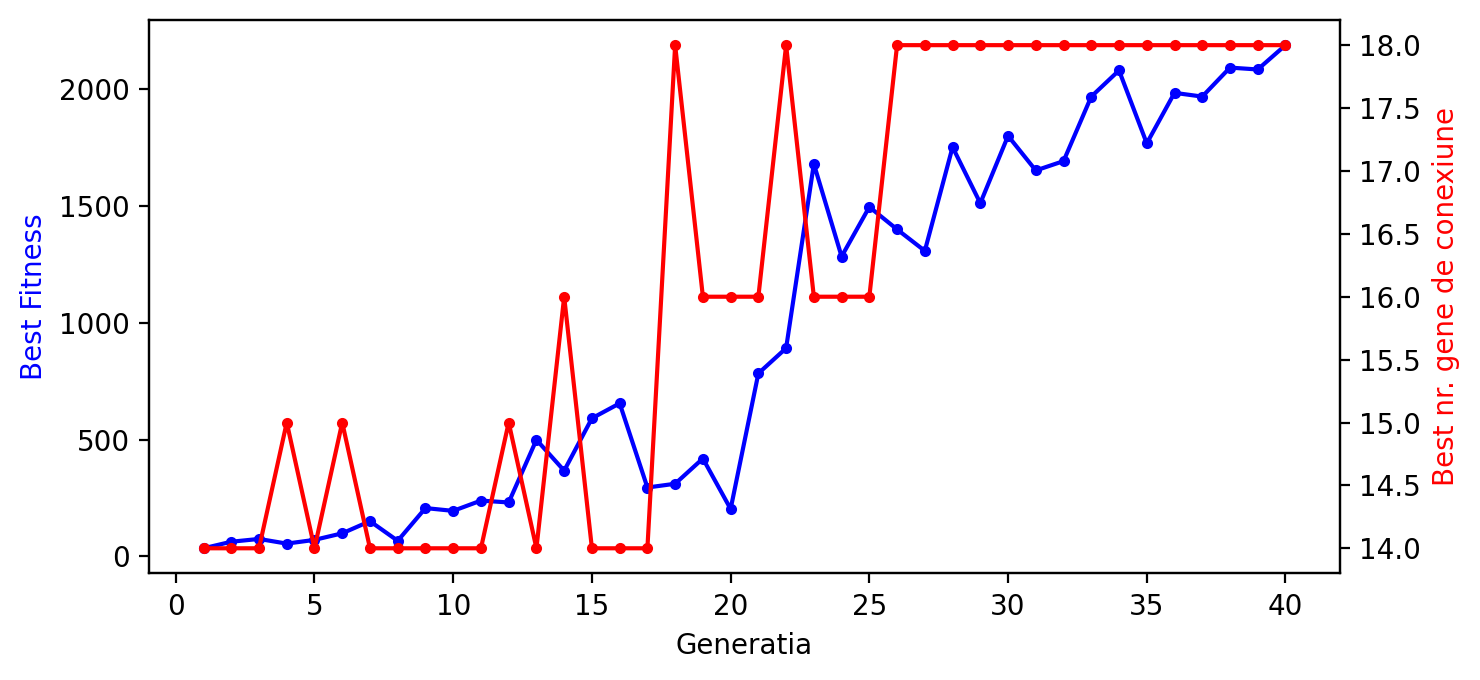
\includegraphics[width=1\textwidth]{images/experiment_inov_connections.png}
	\caption{Progresia fitness-ului celui mai bun membru si a numărului sau de gene de conexiune, in scenariul resetării numerelor de inovație}
	\label{fig:connectionsInov}
\end{figure}


\section{Rezultate Experiment: dezvoltarea comportamentelor de urmărire in prădători}\label{ResultsChassing}
Prin acest experiment am demonstrat ca utilizând NEAT, prădătorii pot să învețe comportamente de urmărire, văzând cu progresia generațiilor si o îmbunătățire a fitness-ului mediu si al celui mai bun membru, in Fig.\ref{fig:averageChassing}.\\
In Fig.\ref{fig:connectionsChassing} putem vedea si faptul ca in același timp se complica si topologia retelei
\begin{figure}[h]
	\centering
	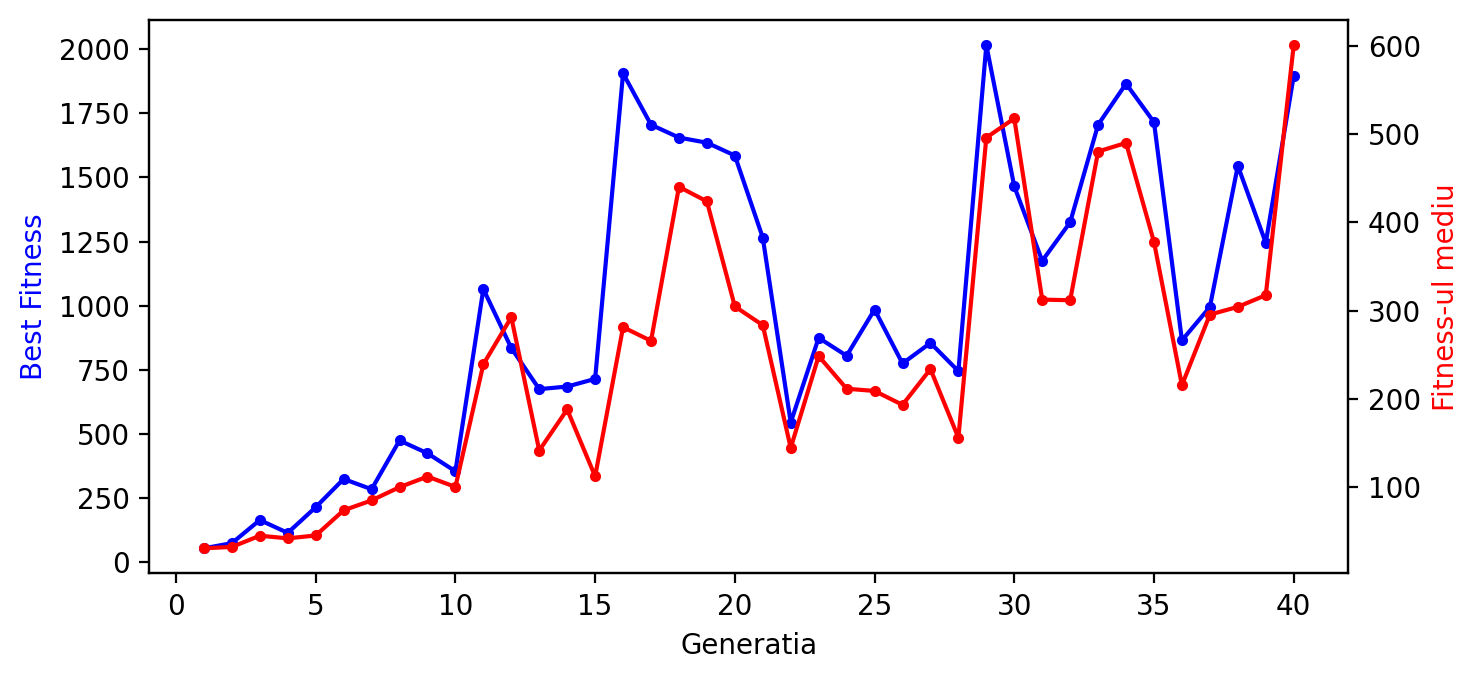
\includegraphics[width=1\textwidth]{images/experiment_chassing_average.png}
	\caption{Progresia fitness-ului celui mai bun prădător si a fitnessului mediu a prădătorilor, in scenariul de dezvoltare al comportamentelor de urmărire}
	\label{fig:averageChassing}
\end{figure}

\begin{figure}[h]
	\centering
	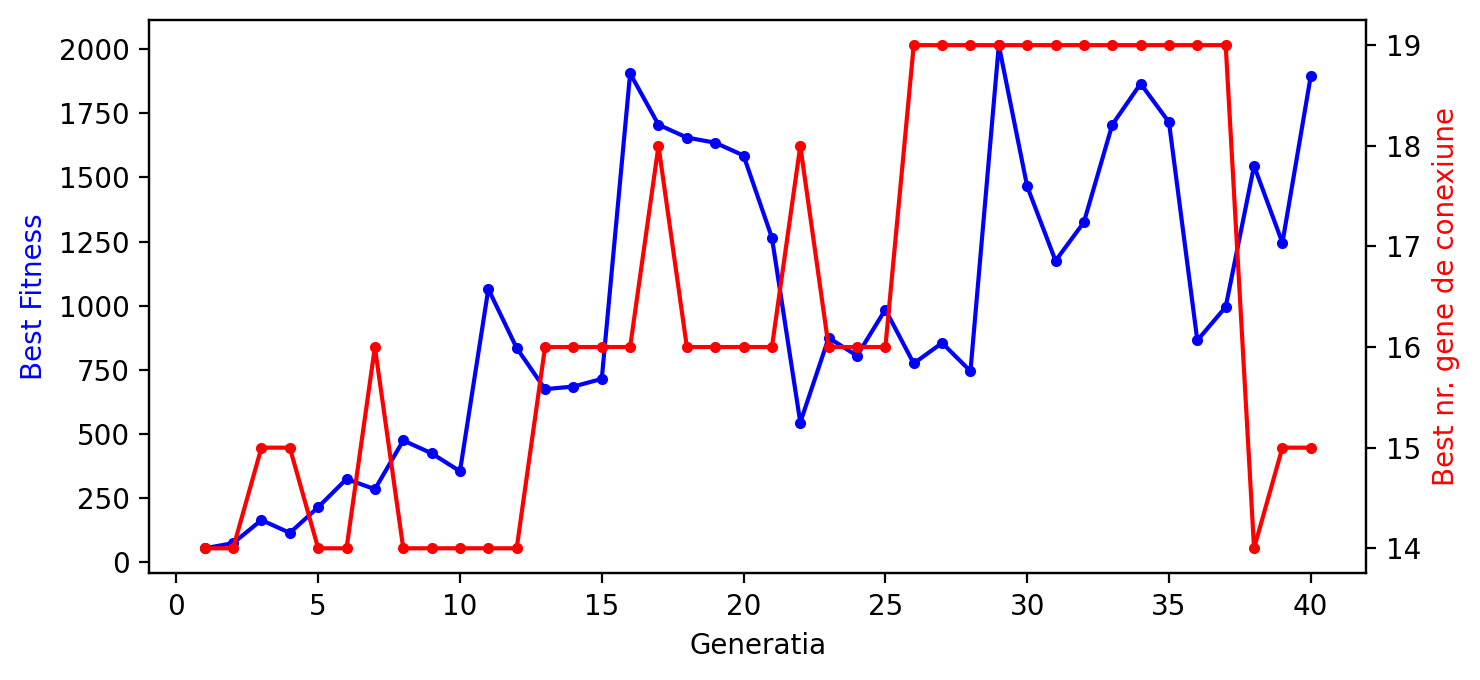
\includegraphics[width=1\textwidth]{images/experiment_chassing_connections.png}
	\caption{Progresia fitness-ului celui mai bun prădător si a numărului sau de gene de conexiune, in scenariul de dezvoltare al comportamentelor de urmărire}
	\label{fig:connectionsChassing}
\end{figure}

\section{Rezultate Experiment: coevoluția prăzii și a prădătorilor}\label{ResultsCoevolution}
Pentru acest experiment, rezultatele sunt dezamăgitoare. Cu parametrii de mediu curent nu am putut stabili o creștere perceptibilă nici pentru fitness-ul prăzii (Fig.\ref{fig:coevPreyAverage}) și nici pentru cel al prădătorilor (Fig.\ref{fig:coevPredatorAverage}).
Se pot vedea spike-uri pe alocuri, ceea ce înseamnă că sunt indivizi care au dezvoltat comportamentele potrivite, dar acestea nu sunt optimizate mai departe în populație.
Putem să vedem asta și prin faptul că apar constant mutații noi, dacă ne uităm la numărul de conexiuni ale celor mai buni membri din ambele populații (Fig.\ref{fig:coevPreyConnections} și Fig.\ref{fig:coevPredatorConnections}).

\begin{figure}[h]
	\centering
	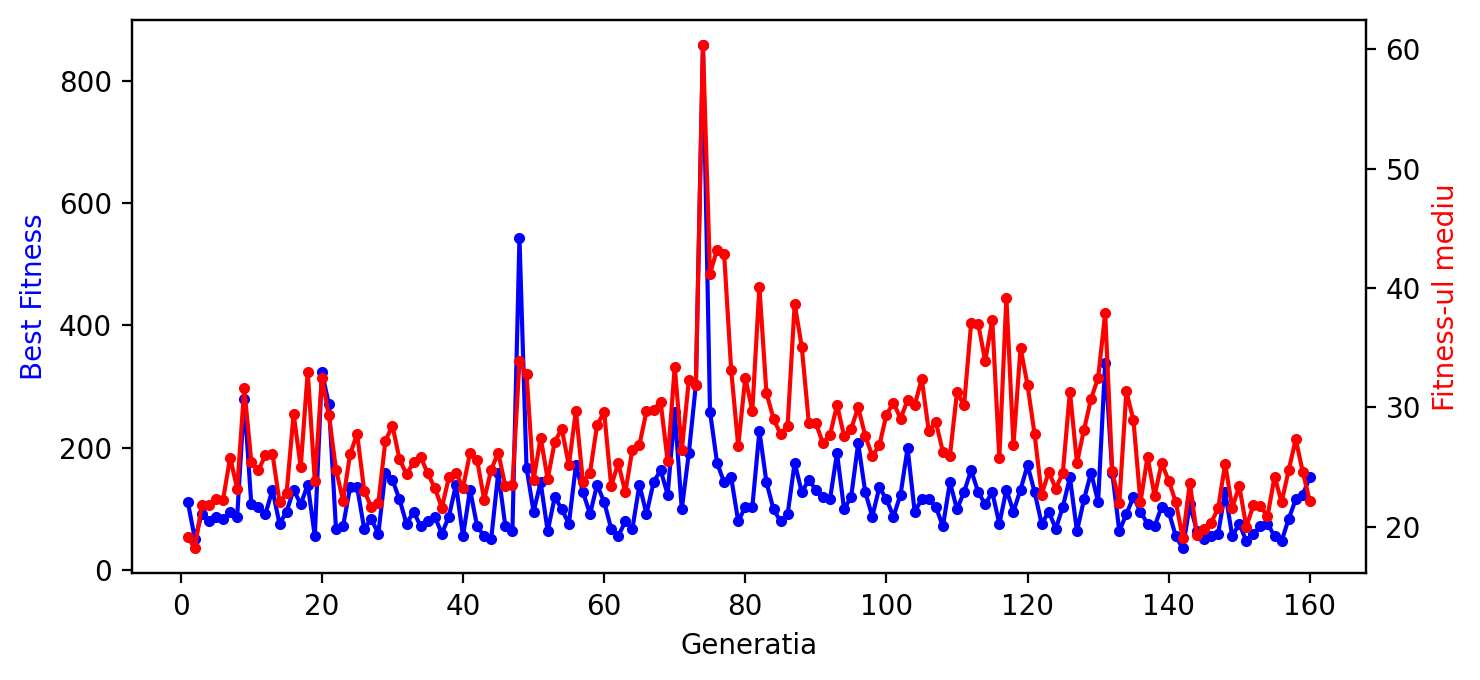
\includegraphics[width=1\textwidth]{images/coevolution_average_prey.png}
	\caption{Progresia fitness-ului celei mai bune prazi si a fitnessului mediu a prăzilor, in experimentul de coevoluție}
	\label{fig:coevPreyAverage}
\end{figure}

\begin{figure}[h]
	\centering
	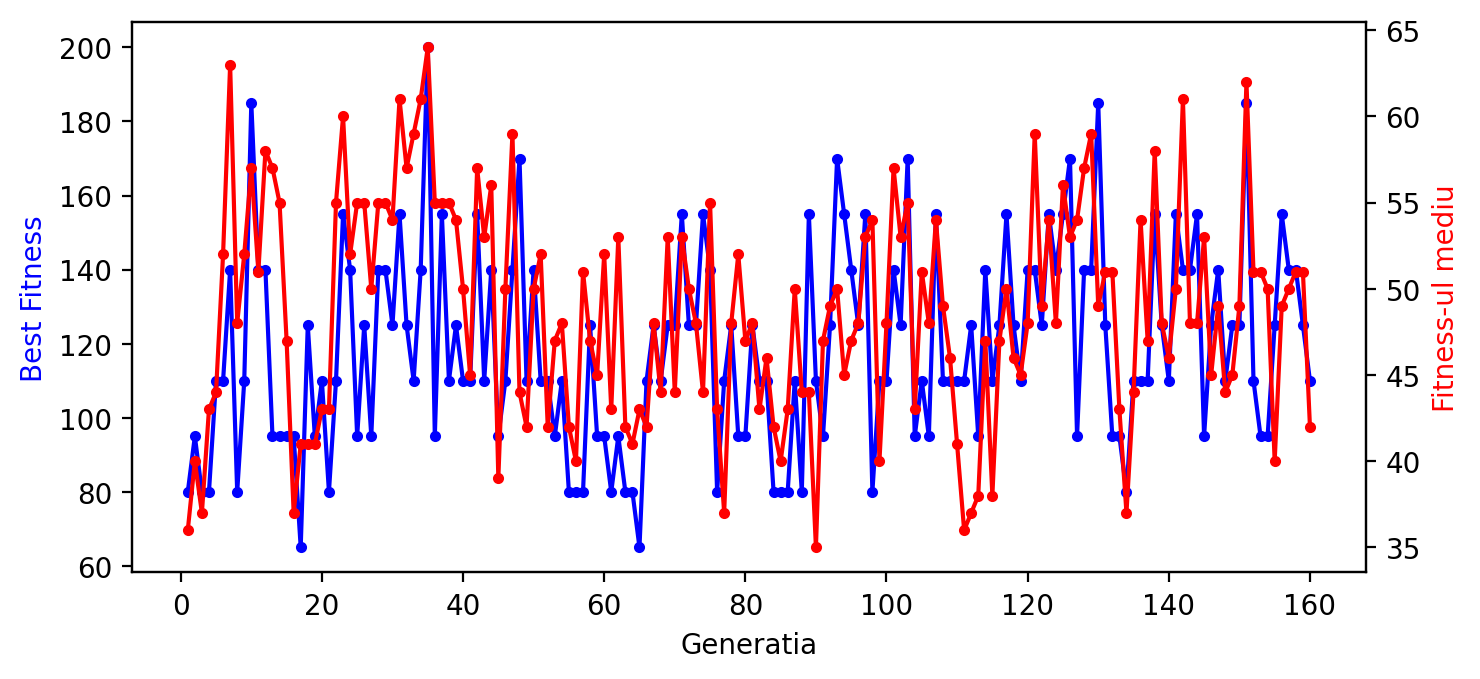
\includegraphics[width=1\textwidth]{images/coevolution_pradator_average.png}
	\caption{Progresia fitness-ului celui mai bun prădător si a fitness-ului mediu al prădătorilor, in experimentul de coevoluție}
	\label{fig:coevPredatorAverage}
\end{figure}

\begin{figure}[h]
	\centering
	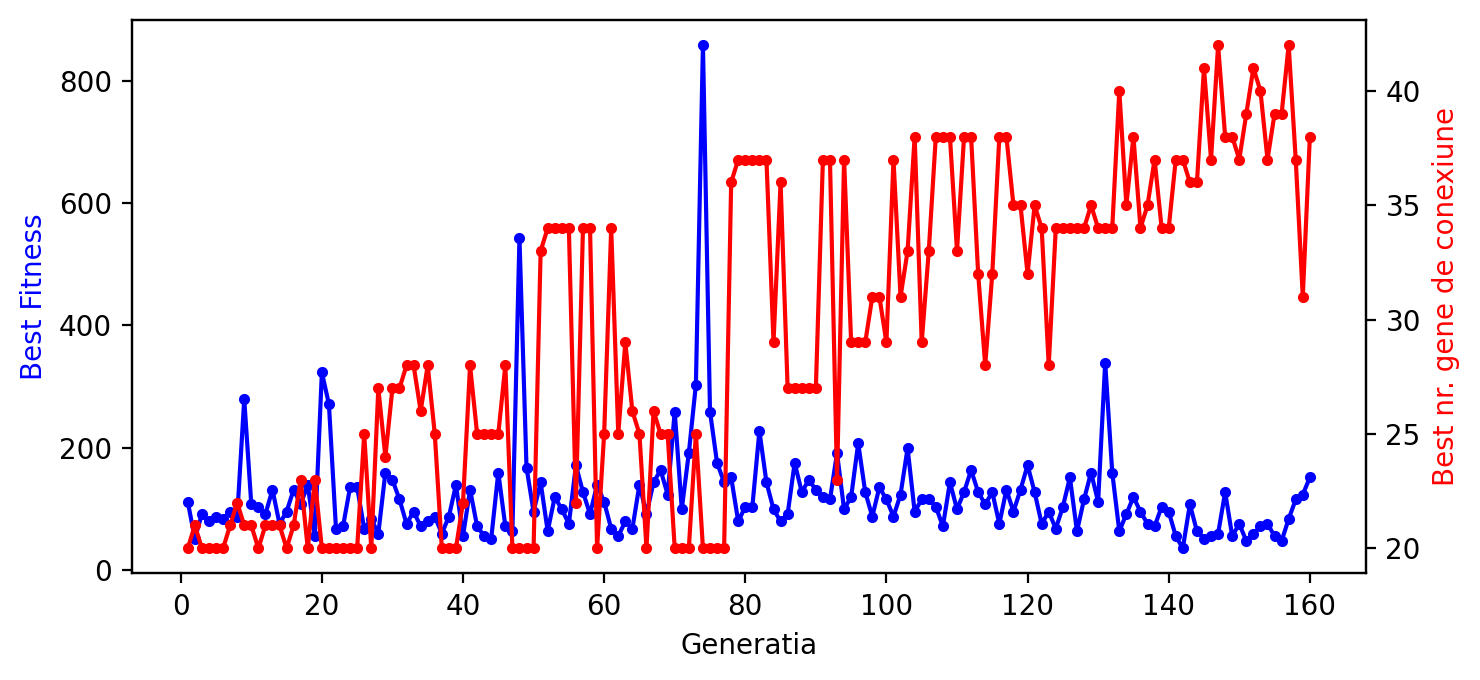
\includegraphics[width=1\textwidth]{images/coevolution_connections_prey.png}
	\caption{Progresia fitness-ului celei mai bune prazi si a numărului ei de gene de conexiune, in experimentul de coevoluție}
	\label{fig:coevPreyConnections}
\end{figure}

\begin{figure}[h]
	\centering
	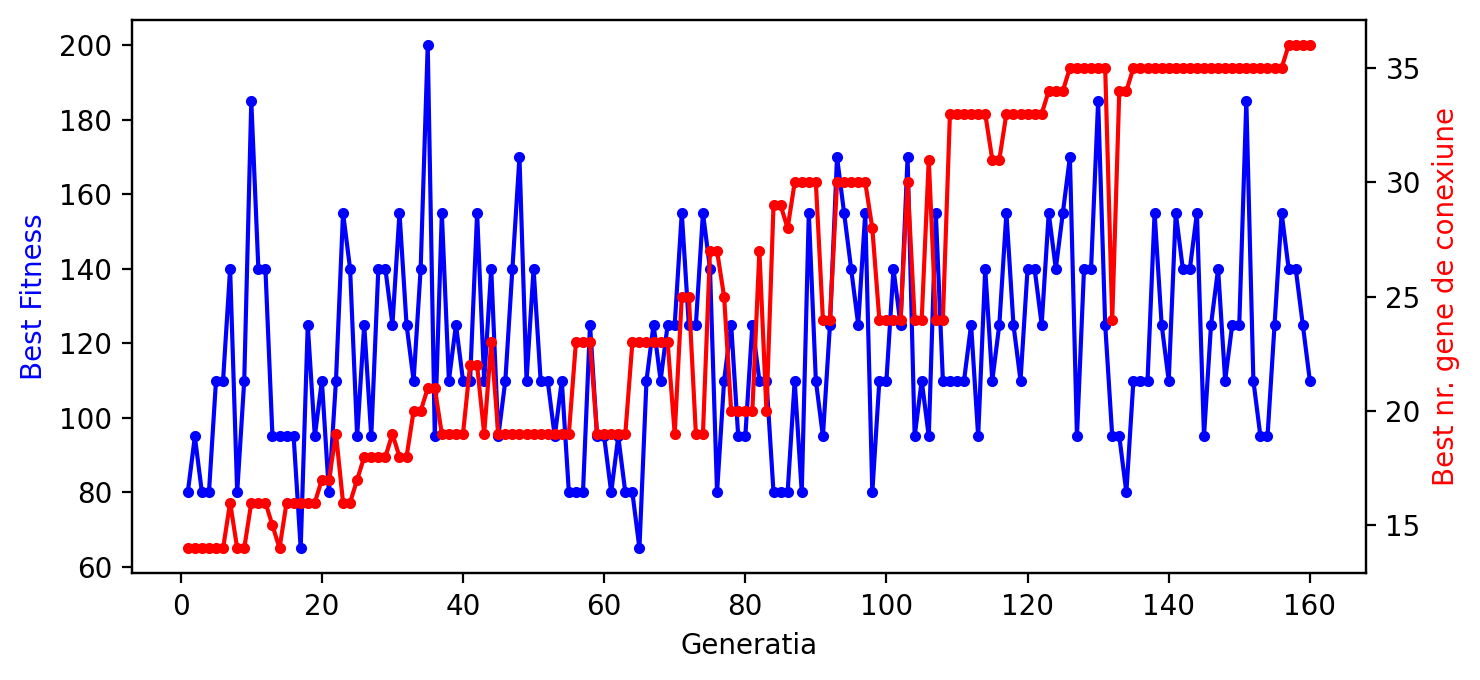
\includegraphics[width=1\textwidth]{images/coevolution_pradator_connections.png}
	\caption{Progresia fitness-ului celui mai bun prădător si a numărului sau de gene de conexiune, in experimentul de coevoluție}
	\label{fig:coevPredatorConnections}
\end{figure}
    
    \chapter*{Concluzii} 
\addcontentsline{toc}{chapter}{Concluzii}
În cadrul acestei teze, am studiat aplicarea algoritmului NEAT in cadrul unui mediu virtual pentru evoluția in mod natural a unor creaturi simulate.\\
În capitolul \ref{NEAT} si capitolul \ref{rtNEAT} am prezentat aspectele teoretice a 2 algoritmi de NeuroEvolutie potriviți pentru scopul nostru, ambii din lucrările lui Kenneth O. Stanley(\cite{NEAT} si \cite{rtNEAT}).\\
La \ref{MediulVirtual} am descris mediul virtual in care va urma rularea simulărilor, si componentele acestuia: "FoodManger", "NeatManager", "Food", "Prey" si "Predator".\\
In \ref{DetaliiImplementare} am detaliat scripturile asociate obiectelor din mediul virtual, precum si detalii proprii de implementare ale NEAT, cu unele îmbunătățiri sugerate in \cite{NeatFAQ}.\\
Prin experimentele din secțiunea \ref{ResultsFowVsFork} am demonstrat ca creaturile de tip "Prey" pot înțelege limitele mediului in care se afla, si pot învața foarte bine comportamente de "grazing", adică de colectare a fragmentelor de energie,
iar prin experimentul din secțiunea \ref{ResultsChassing} am arătat ca prădătorii de asemenea pot înțelege limitele mediului, si pot dezvolta comportamente de urmărire a pradei.\\
Totuși, cu toate ca am reușit sa simulam aceste comportamente esențiale in mod independent, nu am putut crea un mediu echilibrat pentru susținerea coevoluției, după cum am văzut in secțiunea \ref{ResultsCoevolution}.\\
Am observat in timpul simulării indivizi din populația de prada care au învățat sa nu se apropie de prădători, si am văzut si strategii de vânătoare din partea prădătorilor, cum ar fi rotirea in cercuri mai mari pentru a putea lovi prada din punctul ei mort, de la spate.
Însa aceste comportamente nu a reușit sa supraviețuiască de-a lungul generațiilor.\\
Ca arii de dezvoltare pe viitor, ar trebui sa încercam mai multe combinații de parametri in cadrul sistemului controlat de NEAT pentru a putea simula coevoluția. rtNEAT poate fi o varianta încă mai buna a algoritmului pentru acest scop.
Odată ce putem simula coevoluția, ar fi interesant sa schimbam unele din caracteristicile fizice ale indivizilor din populație pentru a vedea ce comportamente noi se pot dezvolta. 
Un exemplu ar fi ca prăzile sa aibă o pereche de "coarne", adică o structura care sa împiedice atacurile din fata. Aceasta idee poate sta si la baza unui eventual joc, unde un jucător poate încerca augmentarea indivizilor sai cu diferite structuri, si sa intre in competiție cu indivizii pregătiți de alt jucător.
Doresc sa mulțumesc profesorului coordonator pentru sfaturile si înțelegerea oferita in cadrul procesului de elaborare a tezei de licența, si profesorilor pe care i-am întâlnit in cadrul facultății in ultimii 3 ani: Mulțumesc pentru tot.

    \printbibliography
\end{document}

